%This document was modified by Asst Prof Adriana Lopes from the latex template "NTU CNYSP Research Report Template (CY1400-CY2001-CY2002)" authored by Karn Watcharasupat.  This is a simplified version to be used by ASE students during their FYP. 


%\documentclass{article}
%\documentclass[12pt,twoside,openright]{report} - with white page between major sections
\documentclass[12pt]{report}

%% Useful packages
\usepackage[a4paper,top=1in,bottom=1in,left=1in,right=1in]{geometry}
\usepackage{amsmath, amssymb, bm}
\usepackage{mathrsfs}
\usepackage{caption}
\usepackage{graphicx}
\usepackage[colorinlistoftodos]{todonotes}
\usepackage[colorlinks=true, allcolors=black]{hyperref}
\usepackage{float}
\usepackage{setspace}
\usepackage{subfigure}
\usepackage{url}
\usepackage{xcolor}
\usepackage{tabularx}
\usepackage{fancybox} %added 
\usepackage[utf8]{vietnam} %added
\usepackage{pifont}
%\usepackage{mathptmx} %Times Font
\usepackage{titlesec}
\titlespacing{\chapter}{0pt}{0pt}{0pt}
\usepackage{fancyhdr}
\usepackage{etoolbox}
\usepackage{appendix}
\usepackage{siunitx}
\usepackage{nomencl}
\newcommand{\nomunit}[1]{%
\renewcommand{\nomentryend}{\hspace*{\fill}#1}}
\makenomenclature
\usepackage{caption}
\usepackage{lipsum}
\usepackage{algpseudocode}
\usepackage{empheq}
\usepackage{mdwlist}
\usepackage{booktabs}
\usepackage{colortbl}
\widowpenalty 10000
\clubpenalty 10000
\usepackage{moresize}

\usepackage[style=apa]{biblatex}
\addbibresource{References.bib}
\DeclareSourcemap{
    \maps[datatype=bibtex]{
        \map{
           \step[fieldsource=title, match=\regexp{\b([A-Z]{2,})\b}, replace={{}{$1}}]
            }
        }
    }
 
\DeclareCaptionType{appfigure}[Figure]
\DeclareCaptionType{apptable}[Table]
\renewcommand{\listappfigurename}{List of Appendix Figures}
\renewcommand{\listapptablename}{List of Appendix Tables}
\renewcommand{\thefigure}{\thechapter-\arabic{figure}}
\renewcommand{\thetable}{\thechapter-\arabic{table}}
\renewcommand{\theappfigure}{\thechapter-\arabic{appfigure}}
\renewcommand{\theapptable}{\thechapter-\arabic{apptable}}
\renewcommand{\contentsname}{Table of Contents}

\newcommand{\chapname}{Chapter }
 
\titleformat{\chapter}[block]
{\bfseries\LARGE\centering}
{}{1em}{}[\rule{\textwidth}{0.3pt}]

\titleformat{\section}
{\bfseries\large}
{\thesection}{1em}{}

\titleformat{\subsection}
{\normalfont\bfseries}
{\thesubsection}{1em}{}

\titleformat{\subsubsection}
{\normalfont\bfseries}
{\thesubsubsection}{1em}{}

\usepackage{fancyhdr}
\usepackage{multirow}
\usepackage{multicol}

\usepackage{placeins}

\makeatletter
\renewcommand*\env@matrix[1][*\c@MaxMatrixCols c]{%
  \hskip -\arraycolsep
  \let\@ifnextchar\new@ifnextchar
  \array{#1}}
\makeatother

\usepackage{enumitem}

\usepackage{listings}
\usepackage{color}
 
\definecolor{codegreen}{rgb}{0,0.6,0}
\definecolor{codegray}{rgb}{0.5,0.5,0.5}
\definecolor{codepurple}{rgb}{0.58,0,0.82}
\definecolor{backcolour}{rgb}{0.95,0.95,0.95}

\newcommand{\codesize}{\fontsize{10pt}{11pt}\selectfont}

\lstdefinestyle{mystyle}{
    backgroundcolor=\color{backcolour},   
    commentstyle=\color{codegreen},
    keywordstyle=\color{magenta},
    numberstyle=\tiny\color{codegray},
    stringstyle=\color{codepurple},
    basicstyle=\ttfamily\codesize,
    breakatwhitespace=true,         
    breaklines=true,                 
    captionpos=b,                    
    keepspaces=false,                 
    numbers=left,                    
    numbersep=5pt,                  
    showspaces=false,                
    showstringspaces=false,
    showtabs=false,                  
    tabsize=2,
    showlines = true,
    fontadjust = true,
    framexleftmargin = 10 pt,
    resetmargins = true,
    basewidth = 0.5em
}
 
\lstset{style=mystyle}

\makeatletter
\setlength{\@fptop}{0pt}
\makeatother

\setlength{\floatsep}{0pt}

\newenvironment{Figure}
  {\noindent\minipage{\linewidth}}
  {\endminipage}

\setcounter{secnumdepth}{5}

\hyphenpenalty 10000
\usepackage{multicol}
 
%%%%%%%%% MATHEMATICS SHORTHANDS %%%%%%%%%%%%%%%%%%%% 

\newcommand{\C}{\mathbb{C}}
\newcommand{\R}{\mathbb{R}}
\newcommand{\Z}{\mathbb{Z}}
%\renewcommand{\d}{\mathrm{d}} %Vĩnh biệt cụ gây lỗi
\renewcommand{\bf}[1]{\mathbf{#1}}

\newcommand{\argmax}[1]{\underset {#1}{\operatorname{arg\,max}}}

\newcommand{\kurt}{\mathrm{kurt}}
\newcommand{\round}{\operatorname{round}}

\newcommand{\E}{\operatorname{E}}
\newcommand{\cov}{\operatorname{cov}}
\newcommand{\pcov}{\operatorname{pcov}}

\newcommand*{\vertbar}{\rule[-1ex]{0.5pt}{2.5ex}}
\newcommand*{\horzbar}{\rule[.5ex]{2.5ex}{0.5pt}}

\setlength{\nomlabelwidth}{3cm}
\setlength{\nomitemsep}{-0.5\parsep}

\usepackage{makecell}
\usepackage{emptypage}

\newcolumntype{R}{>{\raggedleft\arraybackslash}X}
\newcolumntype{L}{>{\raggedright\arraybackslash}X}
\newcolumntype{C}{>{\centering\arraybackslash}X}

\usepackage{textcomp}

%
%\usepackage{background}

%\SetBgScale{1}
%\SetBgContents{\parbox{10cm}{%
%  \Huge Draft:  \today\\[14cm]\rotatebox{180}{\Huge Draft:  %\today}}}
%\SetBgColor{gray}
%\SetBgAngle{270}
%\SetBgOpacity{0.1}
%

%%%%%%%%%%%%%%%%%%%%%%%%%%%%%%%%%%%%%%%%%%%%%%%%%%%%%

\begin{document}
\sloppy
%==== FRONT PART====
\newpage
% \clearpage
 \thispagestyle{empty}

%\thisfancypage*{\setlength{\fboxsep}{15pt}\Ovalbox}{}
\thisfancyput*(8.53cm,-11.5cm){\setlength{\unitlength}{2.54cm}\fancyoval(7.05,9.45)}
 \newcommand*{\Arialfont}{\fontfamily{phv}\selectfont}

\begin{titlepage}
\begin{figure}[!t]
\centering

\includegraphics[width = 4.2in]{Title/download.jpg}
\caption*{}
\end{figure}

\centering
\fontsize{16}{20}\selectfont\textbf{BÁO CÁO MÔN CÁC THÀNH PHẦN PHẦN MỀM}\\[1in]
\fontsize{24}{20}\selectfont\textbf{DESIGN PATTERNS}\\[1in]
    \begin{center}
		\setstretch{1.5}
		\fontsize{14}{20}\selectfont
		\textit{Người hướng dẫn}: 
		    \textbf{Thầy QUẢN THÁI HÀ}\\
		\textit{Người thực hiện}:
		    \textbf{TRẦN NAM KHÁNH - 20001559}\\
		    \textbf{NGUYỄN ANH NGUYỄN - 19000458}\\
		\textit{Lớp}: \textbf{MAT3372 6CLCMTKHTT}\\
	\end{center} \textbf{------------}\\[1in]
	    

\Large{\textbf{HÀ NỘI, NĂM 2022}}\\
\newpage
\end{titlepage}

%\begingroup
%\let\cleardoublepage\clearpage
\pagenumbering{roman}
\pagestyle{fancy}
\fancyhf{}
\cfoot{\thepage}
%\endgroup

%%=== FRONT PART ===
%=== ABSTRCT ===

%\begin{center}
\chapter*{Abstract}
\rhead{Abstract}
%\end{center}
\addcontentsline{toc}{chapter}{Abstract}
%===============================
% ABSTRACT GOES HERE - 250 words limit
%===============================
Vivamus non vehicula tortor. Aenean tincidunt vel nisi id tincidunt. Aliquam eget sollicitudin ipsum. Curabitur quis malesuada magna. Integer nec condimentum sapien. Donec finibus rutrum tellus vel feugiat. Fusce auctor lectus id nunc dignissim, et ultricies eros volutpat. Pellentesque condimentum sed mi et placerat. Morbi semper, erat vitae sodales lobortis, orci enim viverra urna, et mollis mi dui ut ante. Vestibulum sodales lacinia scelerisque. Donec ut augue tellus. Etiam sit amet lacinia ipsum. Morbi commodo, sem sollicitudin dictum fringilla, libero quam varius erat, vel elementum felis velit ut elit. Fusce at sagittis eros. Phasellus tempor ullamcorper massa, consectetur scelerisque purus facilisis in. Vestibulum tempus eros vel sapien rutrum ullamcorper. Fusce at facilisis risus. Donec porttitor augue eu quam tempor, eget cursus risus commodo. Pellentesque sollicitudin, ipsum in tincidunt sagittis, nibh metus ultrices eros, egestas iaculis arcu justo non lectus. Praesent mollis orci ac sodales mollis. Sed suscipit sollicitudin ex id volutpat. Praesent laoreet molestie cursus. Nam dapibus dapibus bibendum. Donec maximus, velit non commodo porttitor, eros lacus ultrices ante, nec interdum purus mauris quis turpis. Nam dapibus quis lacus sed finibus. Aliquam venenatis, ex sit amet suscipit tempor, leo metus porta nulla, a egestas dui mi non risus. Duis vel libero ut mauris sodales cursus nec nec eros. Donec accumsan justo dolor. Quisque varius sem id dui dignissim, sed porta massa sodales. Nulla facilisi. Phasellus id metus ut enim eleifend volutpat. Fusce iaculis sodales tincidunt. Fusce quis convallis justo. Phasellus elementum, felis vel ultrices ultricies, ex nulla euismod justo, et.
%===============================
\\
\par
\textbf{Keywords:} Blind source separation, Independent component analysis, Independent vector analysis, Sparse component analysis, Automatic speech recognition, Android application development.

%=== END OF ABSTRACT ===

%\newpage

%%=== FRONT PART ===
%=== ABSTRCT ===

%\begin{center}
\chapter*{Graphical Abstract}
\rhead{Graphical Abstract}
%\end{center}
\addcontentsline{toc}{chapter}{Graphical Abstract}
%===============================
% Significance Statement goes here - 100 words limits
%===============================

Proin semper mauris arcu, at sodales dolor lobortis eu. Vestibulum non tempus nibh. Proin id mauris tincidunt, hendrerit ipsum at, placerat lacus. Proin ac malesuada mauris. Ut justo arcu, euismod ac magna sit amet, rutrum gravida sapien. Vestibulum efficitur sodales mattis. Mauris ornare leo nec elit fermentum scelerisque. Nullam nec augue sed ex fringilla sagittis. Suspendisse tincidunt sollicitudin tortor eget vehicula. Sed volutpat scelerisque augue sit amet sodales. Donec eget nisi facilisis, viverra magna ac, cursus purus. Mauris eget augue sit amet lectus tempus lacinia eget eu nisi. Morbi rutrum eros non sapien euismod, id sagittis ipsum sagittis. Phasellus eget.


\begin{figure}[h]
\centering
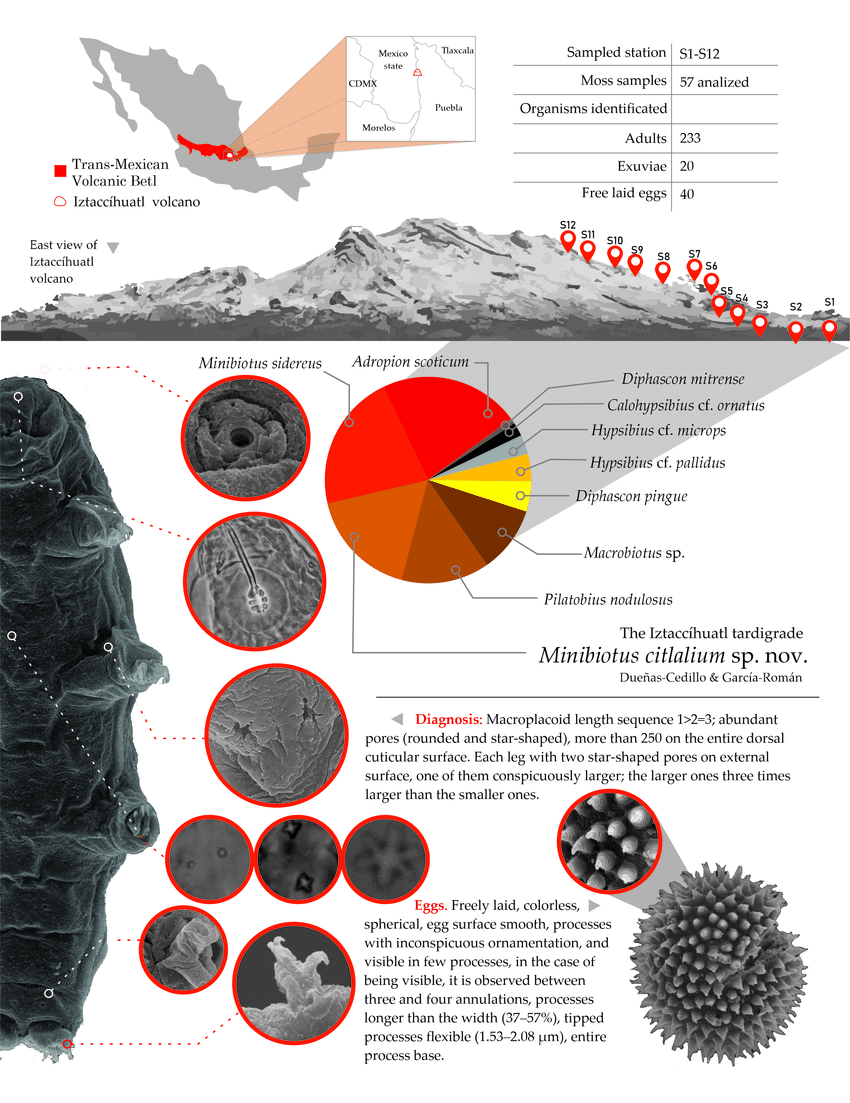
\includegraphics[width=0.8\textwidth]{fig/Graphical-Abstract-example.png}
\end{figure}
%===============================

%=== END OF GRAPHICAL ABSTRACT ===

%\newpage

%%=== FRONT PART ===
%=== ACKNOWLEDGEMENT ===

%\begin{center}
\chapter*{Acknowledgement}
\rhead{Acknowledgement}
%\end{center}
\addcontentsline{toc}{chapter}{Acknowledgement}

Lorem ipsum dolor sit amet, consectetur adipiscing elit, sed do eiusmod tempor incididunt ut labore et dolore magna aliqua. Ut enim ad minim veniam, quis nostrud exercitation ullamco laboris nisi ut aliquip ex ea commodo consequat. Duis aute irure dolor in reprehenderit in voluptate velit esse cillum dolore eu fugiat nulla pariatur. Excepteur sint occaecat cupidatat non proident, sunt in culpa qui officia deserunt mollit anim id est laborum.


%=== END OF ACKNOWLEDGEMENT  ===

%\newpage
%\setcounter{tocdepth}{2}

\tableofcontents
\rhead{Table of Contents}
\newpage

%\include{Front/Nomenclature}
%\newpage

\renewcommand{\listfigurename}{Lists of Figures}
%\rhead{Lists of Figures}
%\listoffigures 
%\addcontentsline{toc}{chapter}{Lists of Figures}

\newpage


%\listoftables 
%\addcontentsline{toc}{chapter}{Lists of Tables}
%\rhead{Lists of Tables}
%\newpage

\rhead{}

%==== MAIN PART ====
\pagenumbering{arabic}

\lhead{Introduction}
%=== INTRODUCTION ===
%Introduction provides background information explaining the theory, processes, aims or hypothesis and rationale for conducting the research project. 

\chapter{1. Giới thiệu tổng quan về Design Pattern}
Trong kĩ thuật phần mềm, \textbf{Design Pattern} là giải pháp chung có thể lặp lại cho những vấn đề thường xảy ra khi thiết kế phần mềm. Design Pattern không phải là một thiết kế hoàn chỉnh mà chuyển hóa trực tiếp thành code. Nó là một khuôn mẫu được đúc kết từ những người đi trước nhằm giải quyết vấn đề mà có thể được sử dụng trong những trường hợp khác nhau

\section{Lợi ích của Design Pattern}
Design Pattern có thể tăng tốc quá trình phát triển bằng cách cung cấp các mô hình phát triển đã được kiểm nghiệm, chứng minh. Thiết kế phần mềm hiệu quả đòi hỏi các vấn đề đáng kể có thể không hiện hữu cho đến khi đến bước triển khai sau này. Việc sử dụng lại các design pattern giúp ngăn chặn các vấn đề nghiêm trọng và cải thiện kĩ năng đọc code cho lập trình viên và kiến trúc sư quen thuộc với các pattern\\[0.1in]
Thông thường, mọi người chỉ hiểu cách để áp dụng một số kĩ thuật thiết kế phần mềm vào những vấn đề nhất định. Những kĩ thuật này khó để áp dụng với những vấn đề ở tầm rộng hơn. Design Pattern cung cấp một giải pháp chung, được ghi lại ở định dạng không bị bó chặt với một vấn đề cụ th \\[0.1in]
Hơn nữa, các design pattern được cải tiến theo thời gian, làm chúng trở nên mạnh mẽ hơn so với các thiết kế đặc biệt

\section{Creational design pattern}
\begin{figure}[!htb]
    \centering
    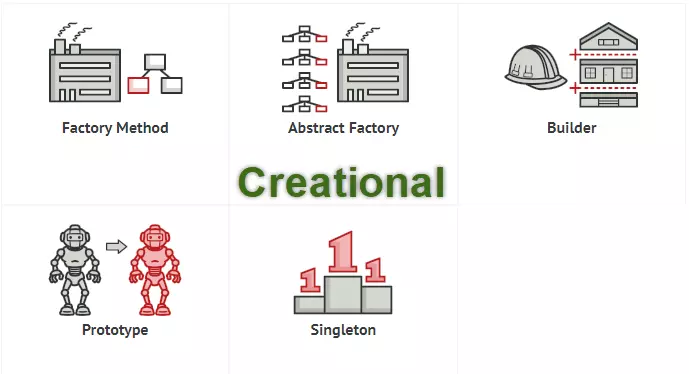
\includegraphics[width=\textwidth]{fig/Introduction/creational.png}
\end{figure}\newpage
Những design pattern này có thiên hướng khởi tạo lớp:
\begin{itemize}
    \item \textbf{Abstract Factory}: Tạo thực thể cho một số họ của các lớp
    \item \textbf{Builder}: Tách biệt cách dựng đối tượng và đối tượng được tạo ra
    \item \textbf{Factory Method}: Tạo thực thể cho mốt số lớp dẫn xuất
    \item \textbf{Object Pool}: Kiểm soát tài nguyên bằng việc tài sử dụng những đối tượng không dùng đến nữa
    \item \textbf{Prototype}: Một thực thể được khởi tạo đầy đủ được dùng để sao chép hoặc nhân bản
    \item \textbf{Singleton}: Một lớp mà chỉ một thực thể duy nhất có thể tồn tại
\end{itemize}

\section{Structural design patterns}
\begin{figure}[!htb]
    \centering
    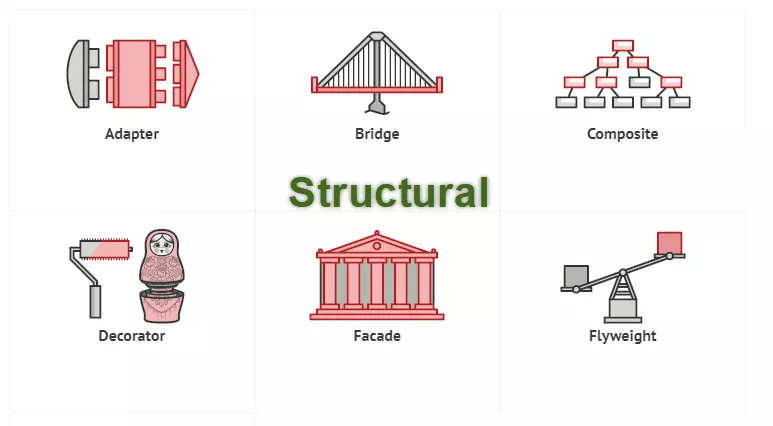
\includegraphics[width=\textwidth]{fig/Introduction/structural.png}
\end{figure}
Những design pattern này có thiên hướng liên kết giữa lớp và đối tượng với nhau:
\begin{itemize}
    \item \textbf{Adapter}: Kết nối Interface của nhiều lớp khác nhau
    \item \textbf{Bridge}: Tách biệt Interface của đối tượng với cách mà nó được triển khai
    \item \textbf{Composite}: Một cấu trúc cây của các đối tượng đơn giản và đối tượng composite
    \item \textbf{Decorator}: Thêm hành vi cho các đối tượng một cách linh động
    \item \textbf{Facade}: Một lớp đơn lẻ đại diện cho cả một hệ thống con
    \item \textbf{Flyweight}: Tái sử dụng đối tượng tương tự đã tồn tại để tối ưu bộ nhớ
    \item \textbf{Proxy}: Một đối tượng đại diện cho một đối tượng khác
\end{itemize}

\section{Behavioral design patterns}
\begin{figure}[!htb]
    \centering
    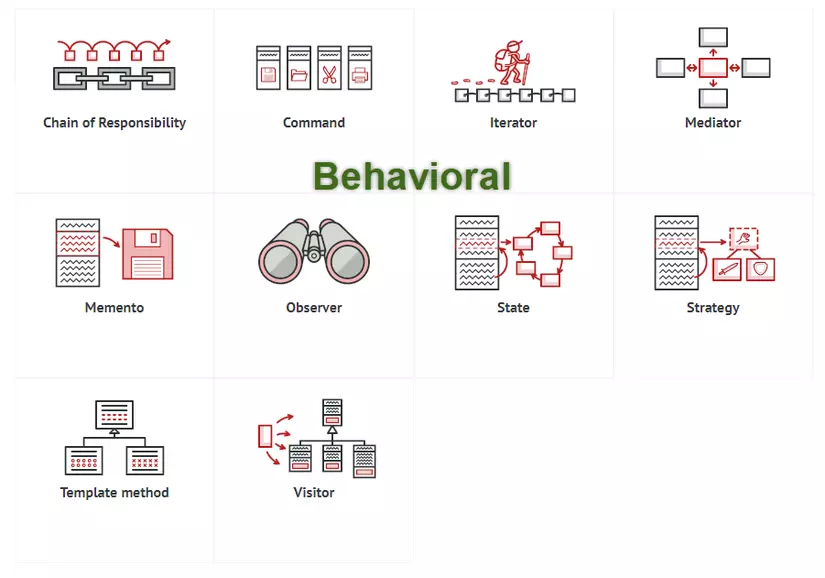
\includegraphics[width=\textwidth]{fig/Introduction/behavioral.png}
\end{figure}
Những design pattern này có thiên hướng giao tiếp giữa các đối tượng
\begin{itemize}
    \item \textbf{Chain of responsibility}: Một cách truyền yêu cầu tới một chuỗi các đối tượng
    \item \textbf{Command}: Đóng gói một lệnh dưới dạng một đối tượng
    \item \textbf{Interpreter}: Một cách bao gồm các yếu tố ngôn ngữ trong chương trình
    \item \textbf{Iterator}: Truy cập tuần tự các phần tử của một tập hợp
    \item \textbf{Mediator}: Định nghĩa cách giao tiếp đơn giản giữa các lớp
    \item \textbf{Memento}: Lưu giữ và khôi phục trạng thái bên trong của đối tượng
    \item \textbf{Null Object}: Thiết kế để hoạt động như một giá trị mặc định của một đối tượng
    \item \textbf{Observer}: Một cách để thông báo sự thay đổi tới một số lớp
    \item \textbf{State}: Thay đổi hành vi đối tượng khi trạng thái của nó thay đổi
    \item \textbf{Strategy}: Đóng gói một thuật toán bên trong một lớp
    \item \textbf{Template method}: Trì hoãn các bước chính xác của thuật toán cho một lớp con
    \item \textbf{Visitor}: Định nghĩa các thao tác tới một lớp mà không làm thay đổi
\end{itemize}


%=== END OF INTRODUCTION ===
\newpage




\lhead{Design Pattern}
\rhead{Facade Pattern}
%=== Materials and Methods ===
\chapter{2. Facade Pattern}
\section{Đặt vấn đề - Rạp hát tại gia}
 Trước khi chúng ta đi chi tiết vào Facade Pattern, hãy tưởng tượng việc xây dựng rạp hát cho ngôi nhà thân yêu của mình\\[0.15in]
 Sau dày công nghiên cứu, cuối cùng ta có được một hệ thống hoàn chỉnh với một đĩa DVD, máy chiếu kỹ thuật số, màn hình tự động và cả một chút bỏng ngô nữa được mô tả trong hình dưới:

%Adding a figure
\begin{figure}[!htb]
    \centering
    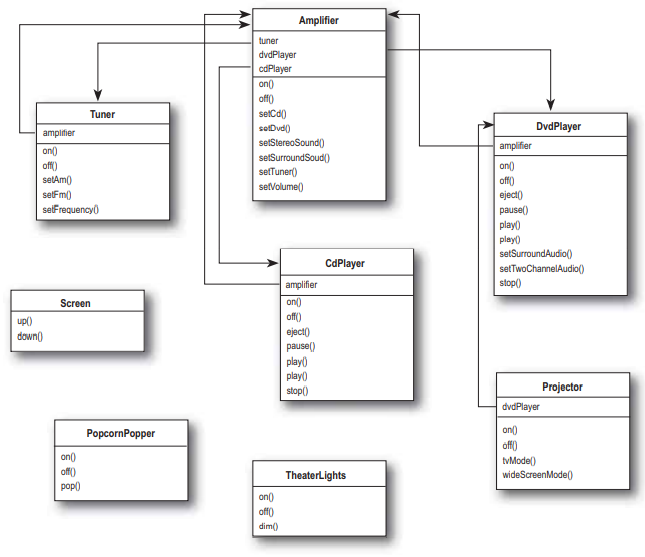
\includegraphics[width=\textwidth]{fig/Facade/TheaterSystem.png}/
\end{figure}
\newpage
Lấy 1 chiếc đĩa DVD, pha tách trà và thư giãn. Nhưng mà chờ đã, trước khi xem phim ta cần phải thực hiện những việc sau: bật bắp rang bơ lên, giảm độ sáng, đặt màn hình xuống, bật máy chiếu lên,....  Với việc gọi lớp và phương thức thông thường

\begin{figure}[!htb]
    \centering
    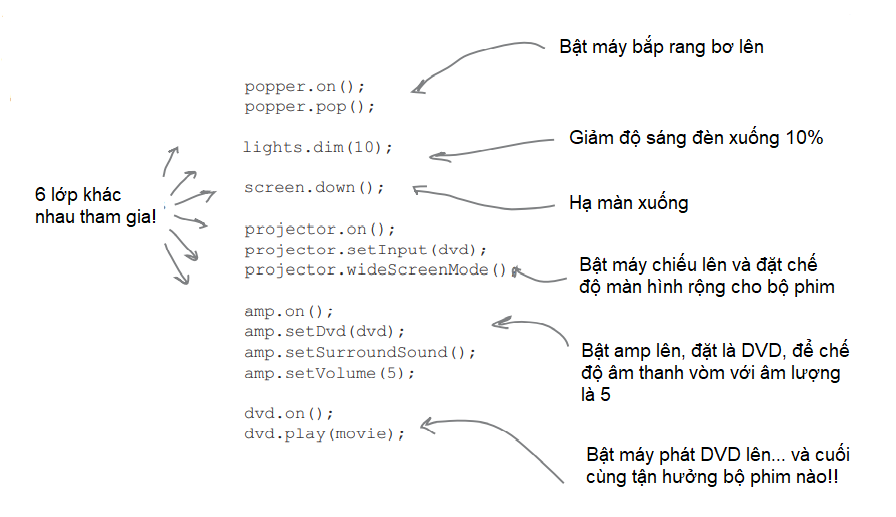
\includegraphics[width=\textwidth]{fig/Facade/TheaterWithClassMethodCalling.png}/
\end{figure}
\textbf{Việc này phát sinh 1 số vấn đề như sau:}\smallskip

- Khi bộ phim kết thúc, làm sao để tắt mọi thứ? Hay phải làm hết những việc này theo chiều ngược lại?\smallskip

- Việc nghe đĩa CD hay Radio cũng phức tạp không kém gì DVD?\smallskip

- Khi nâng cấp hệ thống, chương trình trong Client cũng phải sửa đi\bigskip

\textbf{Facade Pattern} là giải pháp cho những vấn đề trên. Mục đích chính là để giảm độ phức tạp trong hệ thống và đơn giản hóa interface. Không những vậy, Facade thể hiện tính trừu tượng: giấu đi những thứ được triển khai bên trong và chỉ để lại Interface cho Client dễ dàng sử dụng
\newpage
\section{Định nghĩa và Mô hình cấu trúc}
\subsection{Định nghĩa}

\textbf{Facade Pattern} cung cấp một giao diện thống nhất một tập hợp những giao diện trong một hệ thống con. Facade xác định một giao diện ở mức cao để thuận tiện trong việc sử dụng hệ thống con

\subsection{Mô hình cấu trúc}

Mô hình cấu trúc của Facade Pattern được biểu diễn như sau:
\begin{figure}[!htb]
    \centering
    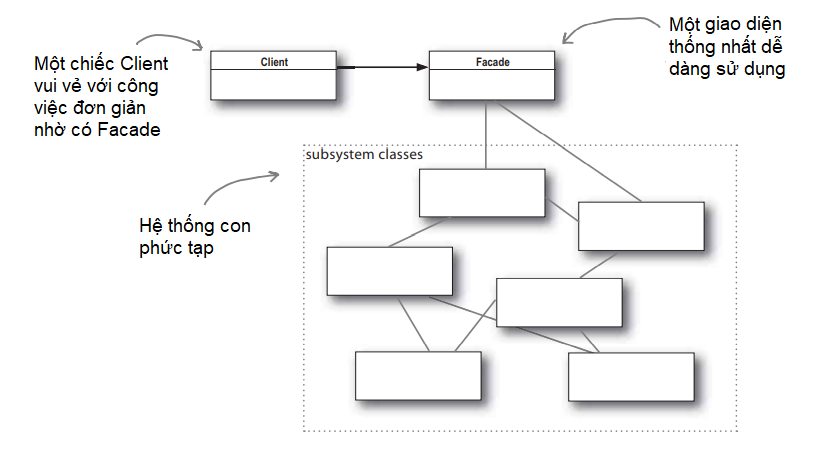
\includegraphics[width=\textwidth]{fig/Facade/FacadeDiagram.png}/
\end{figure}
\newpage
\section{Facade Pattern: Rạp hát - Set ON!}

Nhờ vào mô hình cấu trúc đã được định nghĩa ở trên, ta có thể nâng cấp rạp hát với mô hình như sau:
\begin{figure}[!htb]
    \centering
    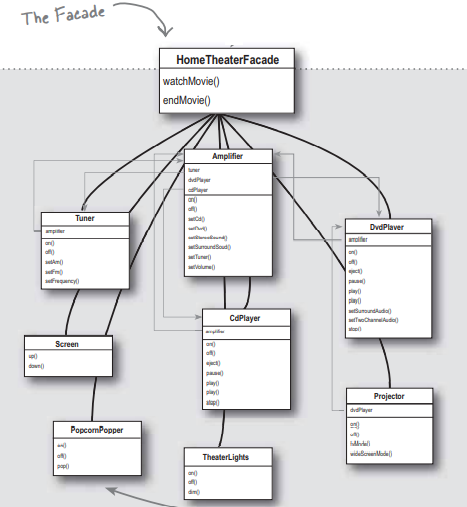
\includegraphics[width=\textwidth]{fig/Facade/TheaterFacade.png}/
\end{figure}

Về mặt ý tưởng, ta sẽ tạo một lớp mới tên là \textbf{HomeTheaterFacade}, nơi chứa một vài phương thức như \textbf{watchMovie()}. Lúc này, lớp Facade sẽ coi những thành phần trong rạp như một hệ thống con và gọi chúng trong phương thức \textbf{watchMovie()}. Client sẽ gọi những phương thức trong lớp Facade, không phải hệ thống con. Nói cách khác, khi cần xem phim thì việc gọi phương thức \textbf{watchMovie()} và phương thức đó sẽ tự động kết nối đến đèn, đầu đĩa DVD, máy chiếu, bộ khuếch đại,...
\newpage
Dưới đây là doạn code minh họa cho lớp HomeTheaterFacade:
\begin{figure}[!htb]
    \centering
    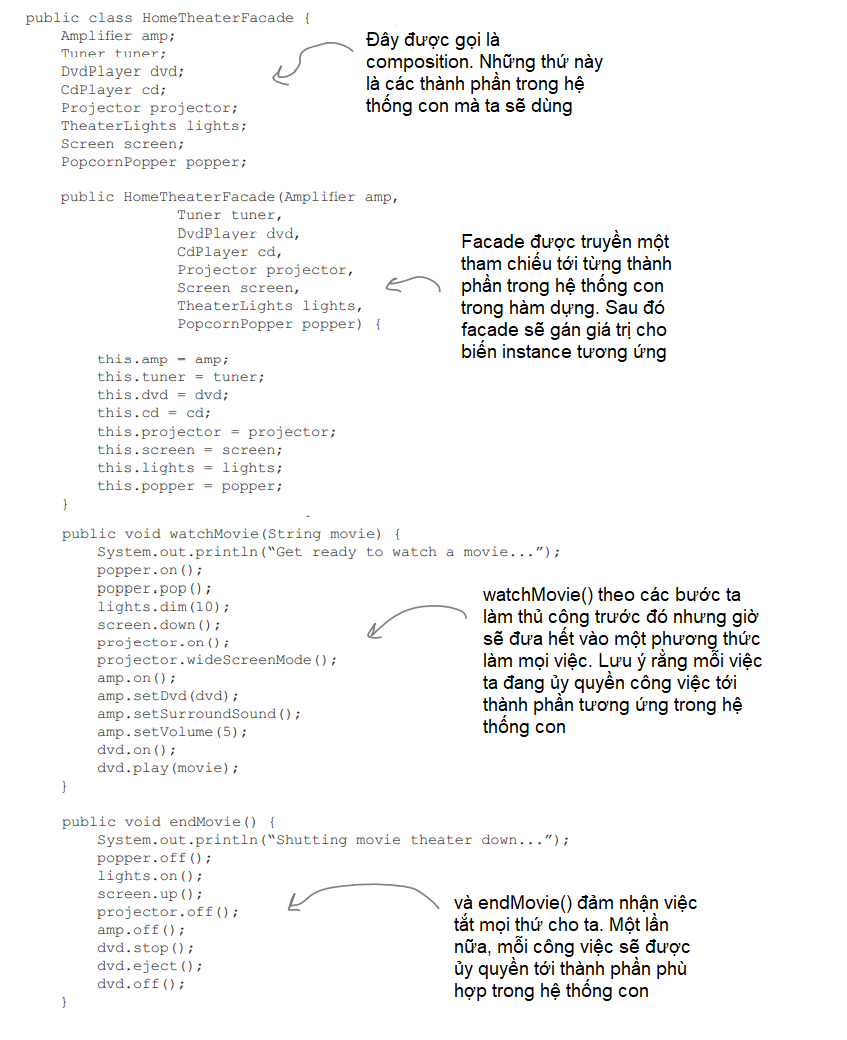
\includegraphics[width=\textwidth]{fig/Facade/HomeTheaterFacade.png}/
\end{figure}
\newpage

Đến giờ thưởng thức phim sau bao công sức:
\begin{figure}[!htb]
    \centering
    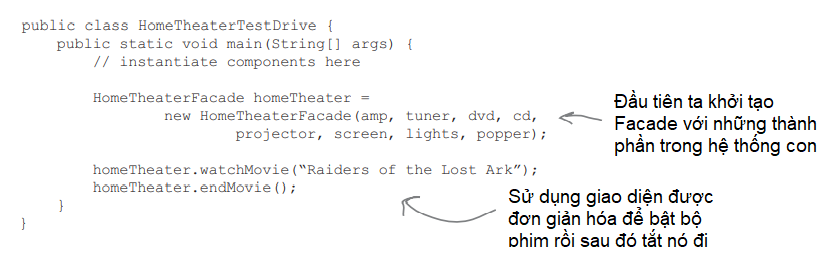
\includegraphics[width=\textwidth]{fig/Facade/TheaterMain.png}/
\end{figure}

\section{Thực tế}

Trong ET++ application framework [WGM88], một ứng dụng có thể được tích hợp sẵn các công cụ duyệt để kiểm tra các đối tượng của nó tại thời điểm chạy. Những công cụ duyệt này được triển khai trong một hệ thống con riêng biệt bao gồm một lớp \textbf{Facade} được gọi là "ProgrammingEnvironment". Những facade này định nghĩa các toán tử như InspectObject và InspectClass để truy cập các trình duyệt\\[0.1in]
Hệ điều hành The Choices [CIRM93] sử dụng facade để hợp thành nhiều framework thành một. Có những phần chính trong Choices là quy trình, không gian lưu trữ và không gian địa chỉ. Ứng với mỗi phần sẽ có một hệ thống con tương ứng, triển khai như một framework hỗ trợ chuyển Choices tới nhiều nền tảng phần cứng khác nhau. 2 trong những hệ thống con có một "representative" (i.e.facade). Những representatives là FileSystemlnterface (không gian lưu trữ) và Domain (không gian địa chỉ)

%=== END OF MM ===
\newpage


\lhead{Design Pattern}
\rhead{Singleton Pattern}
\chapter{3. Singleton Pattern}

\section{Giới thiệu}
\subsection{Đặt vấn đề}
Hầu hết các đối tượng trong một ứng dụng đều chịu trách nhiệm cho công việc của chúng và truy xuất dữ liệu tự lưu trữ (self-contained data) và các tham chiếu trong phạm vi được đưa ra của chúng.Tuy nhiên, có nhiều đối tượng có thêm những nhiệm vụ và có ảnh hưởng rộng hơn, chẳng hạn như quản lý các nguồn tài nguyên bị giới hạn hoặc theo dõi toàn bộ trạng thái của hệ thống.Ví dụ có nhiều máy in trong một hệ thống nhưng chỉ tồn tại duy nhất một Sprinter Spooler(Phần quản lí máy in).\\
Hay giả sử trong ứng dụng có chức năng bật tắt nhạc nền chẳng hạn, khi người dùng mở app thì ứng dụng sẽ tự động mở nhạc nền và nếu người dùng muốn tắt thì phải vào setting trong app để tắt nó, trong setting của app cho phép người dùng quản lí việc mở hay tắt nhạc, và trong trường hợp này sẽ cần sử dụng singleton để quản lí. Chắc chắn chúng ta phải cần duy nhất 1 instance để có thể ra lệnh bật hay tắt, tại sao ? vì đơn giản bạn không thể tạo 1 instance để mở nhạc rồi sau đó lại tạo 1 instance khác để tắt nhạc, lúc này sẽ có 2 instance được tạo ra, 2 instance này không liên quan đến nhau nên không thể thực hiện thực hiện việc cho nhau được,nói cách khác instance nào bật thì chỉ có instance đó mới được phép tắt nên dẫn đến phải cần 1 instance.\\
Để phục vụ nhu cầu kể trên Singleton Pattern đã được tạo ra.
\subsection{Mục đích sử dụng}
Mô hình thiết kế singleton giải quyết các vấn đề bằng cách cho phép nó:
\begin{itemize}
    \item Đảm bảo rằng một class chỉ có một instance
    \item Dễ dàng truy cập instance duy nhất của một class
    \item Kiểm soát sự khởi tạo của instance
    \item Hạn chế số lượng phiên bản
    \item Truy cập một biến toàn cục
\end{itemize}
Mô hình thiết kế singleton mô tả cách giải quyết các vấn đề như:
\begin{itemize}
    \item Ẩn các constructor của một class .
    \item Định nghĩa một hoạt động tĩnh công khai ( getInstance()) trả về thể hiện duy nhất của class.
\end{itemize}

Về bản chất, mô hình Singleton buộc nó phải chịu trách nhiệm đảm bảo rằng nó chỉ được khởi tạo một lần. Một phương thức khởi tạo ẩn — được khai báo private hoặc protected đảm bảo rằng lớp không bao giờ có thể được khởi tạo từ bên ngoài lớp. Hoạt động tĩnh công cộng có thể được truy cập bằng cách sử dụng tên class và tên operation.\\Ví dụ Singleton.getInstance():.

\section{Định nghĩa và mô hình cấu trúc}

\subsection{Định nghĩa}
Singleton là một Design Pattern thuộc nhóm khởi tạo(Creational).Nó đảm bảo rằng một class chỉ có duy nhất một instance được khởi tạo và chỉ có một cách (toàn cầu) để có quyền truy cập vào instance đó.

\subsection{Mô hình cấu trúc}
\begin{figure}[!htb]
    \centering
    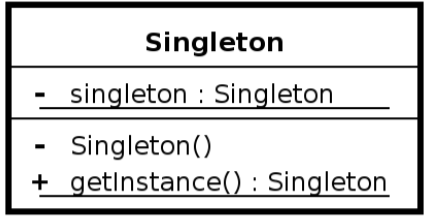
\includegraphics[height=6cm,width=9cm] {fig/Singleton/structure_singleton.png}
    \caption{Mô hình cấu trúc Singleton Pattern}
    \label{fig:structure_singleton}
\end{figure}

-Singleton chỉ liên quan đến một lớp duy nhất (thường không được gọi là Singleton). Lớp đó là một lớp đầy đủ với các thuộc tính và phương thức khác (không được hiển thị).
    
-Lớp có một biến static trỏ đến một thể hiện duy nhất của lớp.
    
-Lớp có một phương thức khởi tạo riêng (để ngăn mã khác khởi tạo lớp) và một phương thức tĩnh cung cấp quyền truy cập vào cá thể đơn lẻ.

\section{Cách cài đặt}
\subsection{Cài đặt chung}
Để cài đặt Singleton Pattern chúng ta cần làm hai bước.\\
Bước 1: Cần để class có duy nhất một instance
\begin{itemize}
    \item Private constructor của class đó để đảm bảo rằng class khác không thể truy cập vào constructor và tạo ra instance mới.
    \item Tạo một biến private static là thể hiện của class đó để đảm bảo rằng nó là duy nhất và chỉ được tạo ra trong class đó thôi.
\end{itemize}
Bước 2: Cung cấp một cách toàn cầu để truy cập tới instance đó
\begin{itemize}
    \item Tạo một public static method trả về instance vừa khởi tạo bên trên, đây là cách duy nhất để class khác có thể truy cập vào instance của class này.
\end{itemize}

Dưới đây là code minh họa cài đặt Singleton Pattern.\\

\begin{figure}[!htb]
    \centering
    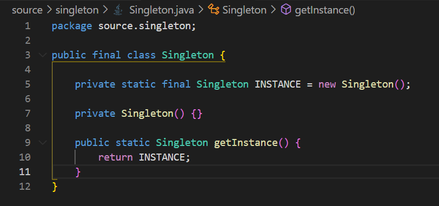
\includegraphics[width=\textwidth]
    {fig/Singleton/singleton_class.png}
    \caption{Singleton class}
    \label{fig:Singleton Class}
\end{figure}

\subsection{Cài đặt cho ví dụ cụ thể}
Dưới đây là ví dụ áp dụng Singleton Pattern.\\
Link code cài đặt:
\url{https://github.com/nanhus/OOP-DesginPatten/tree/master/source/singleton}

\begin{figure}[!htb]
    \centering
    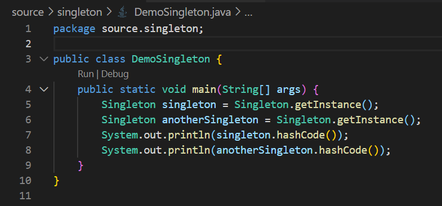
\includegraphics[width=\textwidth]{fig/Singleton/demo_singleton_class.png}
    \caption{Demo Singleton Class}
    \label{fig:demo_singleton_class}
\end{figure}
\begin{figure}[!htb]
    \centering
    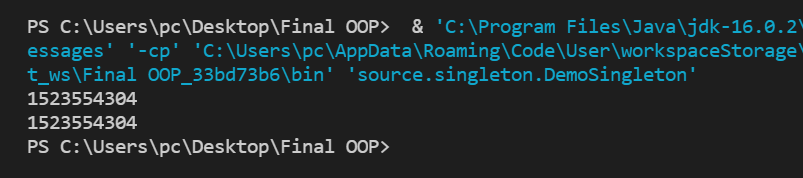
\includegraphics[width=\textwidth]{fig/Singleton/singleton_output.png}
    \caption{Output}
    \label{fig:singleton_output}
\end{figure}
\newpage
Như chúng ta đã thấy output cho ra kết quả là 2 ô nhớ cùng địa chỉ.Như vậy Singleton Pattern đã được cài đặt.

\section{Ví dụ thực tế}
\begin{itemize}
    \item Centralized manager of resources
    \begin{itemize}
        \item Window manager
        \item File system manager
        \item ...
    \end{itemize}
    \item Logger classes
    \item Factories
    \begin{itemize}
        \item Đặc biệt là những vấn đề  IDs
        \item Singleton thường được kết hợp với các mẫu Factory Method và Abstract Factory
    \end{itemize}
\end{itemize}

\newpage


\lhead{Design Pattern}
\rhead{Template Pattern}
\chapter{4. Template Pattern}
\section{Đặt vấn đề - Pha cà phê và Pha trà}
Một số người không thể sống nếu thiếu đi cà phê, một số người không thể sống nếu thiếu đi trà. Việc pha cà phê và pha trà khá giống nhau\smallskip

Công thức làm cà phê:
\begin{itemize}
\item Đun sôi nước
\item Pha cà phê vào nước sôi
\item Rót cà phê vào cốc
\item Thêm đường và sữa
\end{itemize}

Công thức làm trà:
\begin{itemize}
\item Đun sôi nước
\item Ngâm trà trong nước sôi
\item Rót trà vào cốc
\item Thêm chanh
\end{itemize}
Hãy thử pha cà phê và trà bằng code:\\[0.1in]
Cà phê:
\begin{figure}[!htb]
    \centering
    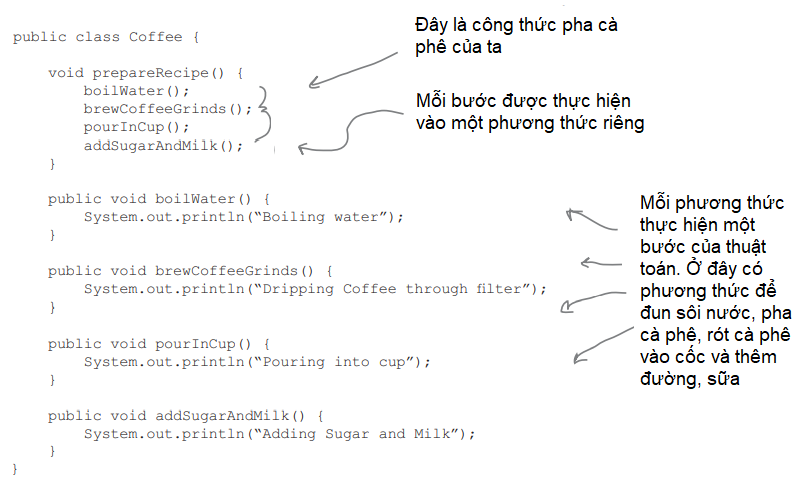
\includegraphics[width=\textwidth]{fig/Template/Coffee.png}/
\end{figure}\\[0.1in]

Trà:
\begin{figure}[!htb]
    \centering
    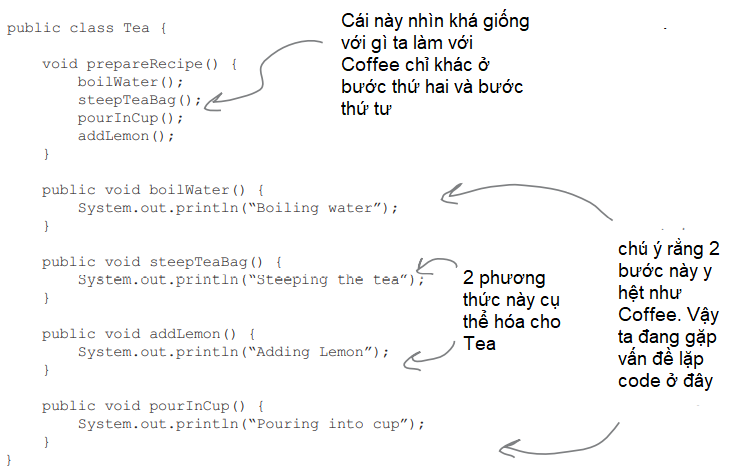
\includegraphics[width=\textwidth]{fig/Template/Tea.png}/
\end{figure}

Rõ ràng có thể thấy code bị dư thừa và lặp lại khá nhiều. Ta phải hạn chế bằng cách nhóm những điểm chung vào một lớp vì cách thức làm cà phê và trà khá tương đồng\\[0.1in]

Lưu ý rằng cả 2 công thức đều được xây dựng trên một thuật toán:
\begin{itemize}
\item Đun sôi nước
\item Dùng nước sôi trích xuất trà / cà phê
\item Đổ thành phẩm vào cốc
\item Thêm gia vị thích hợp
\end{itemize}

Về mặt ý tưởng để cải tiến, ta sẽ tạo một lớp cha tên là \textbf{CaffeineBeverage}. Bên trong lớp này sẽ có một phương thức \textbf{prepareRecipe()} thực hiện thuật toán chung cho cả cà phê lẫn trà\smallskip

Do thuật toán chung có 4 bước nên trong phương thức \textbf{prepareRecipe()} cũng sẽ có 4 phương thức đại diện: \textbf{boilWater()}, \textbf{brew()}, \textbf{pourInCup()}, \textbf{addCondiments()}\smallskip

Do cách trích xuất và thêm gia vị của cà phê, trà là khác nhau nên phương thức \textbf{brew()}, \textbf{addCondiments()} sẽ đánh dấu abstract. Còn lại sẽ được triển khai trong lớp cha
\newpage

Dưới đây là code minh họa cho lớp \textbf{CaffeineBeverage}:

\begin{figure}[!htb]
    \centering
    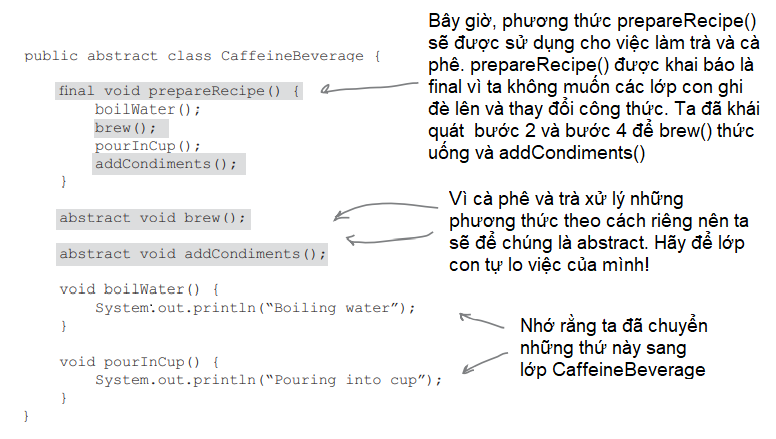
\includegraphics[width=\textwidth]{fig/Template/CaffeineBeverage.png}/
\end{figure}

Đây là code cho 2 lớp Trà và cà phê với cách thiết kế mới:
\begin{figure}[!htb]
    \centering
    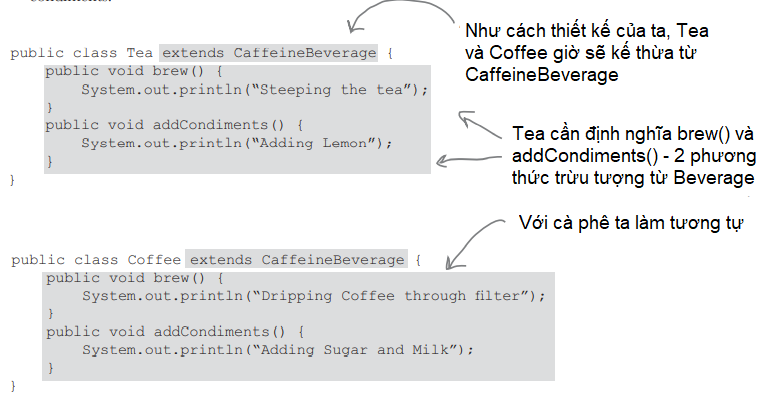
\includegraphics[width=\textwidth]{fig/Template/TeaAndCoffeeNewDesign.png}/
\end{figure}

Tổng kết lại, những gì ta đã làm là cài đặt \textbf{Template Method Pattern}. Phương thức \textbf{prepareRecipe()} được gọi là \textbf{Template Method}\smallskip

Qua ví dụ trên, \textbf{Template Method Pattern} giúp tối đa hóa việc tái sử dụng code giữa các lớp. Hơn nữa, thuật toán sẽ nằm yên một chỗ thuận tiện trong quá trình sửa đổi. Cuối cùng, Template cung cấp một Framework hỗ trợ các loại đồ uống chứa caffeine khác. Đó cũng là mục đích sử dụng chính của \textbf{Template Method Pattern}.

\newpage
\section{Định nghĩa và Mô hình cấu trúc}
\subsection{Định nghĩa}

\textbf{Template Method Pattern} định ra khung xương cho thuật toán trong một phương thức, trì hoãn một số bước tới những lớp con. Template Method cho phép những lớp con tự định nghĩa lại một số bước nhất định mà không làm thay đổi cấu trúc thuật toán

\subsection{Mô hình cấu trúc}

Mô hình cấu trúc của Template Method Pattern được mô tả như sau:

\begin{figure}[!htb]
    \centering
    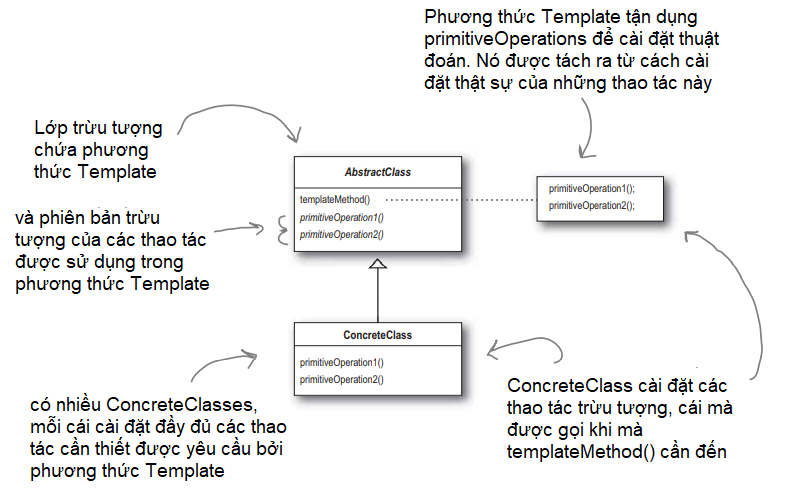
\includegraphics[width=\textwidth]{fig/Template/TemplateDiagram.png}/
\end{figure}

\section{Thực tế}
Template Method Pattern khá là cơ bản đến nỗi nó được thấy ở hầu hết các lớp trừu tượng \\[0.1in]
Dưới đây là những phương thức Template trong bộ thư viện chuẩn của Java:
\begin{itemize}
    \item Tất cả các phương thức không phải trừu tượng của \textbf{java.io.InputStream}, \textbf{java.io.OutputStream}, \textbf{java.io.Reader}, \textbf{java.io.Writer}
    \item Tất cả các phương thức không phải trừu tượng của
    \textbf{java.util.AbstractList}, \textbf{java.util.AbstractSet}, \textbf{java.util.AbstractMap}
\end{itemize}

%=== END OF MM ===
\newpage

\lhead{Design Pattern}
\rhead{Observer Pattern}
\chapter{5.Observer Pattern}

\section{Giới thiệu}
\subsection{Đặt vấn đề}
Chúng ta cần thiết kế và xây dựng một hệ thống phần mềm cho một trạm quan sát thời tiết. Dữ liệu của hệ thống được xây dựng thông qua một đối tượng gọi là WeatherData - đóng vai trò theo dõi điều kiện thời tiết hiện tại (nhiệt độ, độ ẩm, áp suất).\\
Yêu cầu ứng dụng cung cấp 3 phần tử màn hình hiển thị:
\begin{itemize}
    \item CurrentConditionDisplay
    \item StatsisticsDisplay
    \item ForcastDisplay
\end{itemize}
Tất cả sẽ được cập nhật theo thời gian thực mỗi khi đối tượng WeatherData lấy được dự liệu mới nhất.\\
Ngoài ra, trạm quan sát cũng muốn "public" những API để những lập trình viên khác có thể viết ra những màn hình hiển thị thời tiết của riêng họ.\\
Trong trường hợp trên, để có một thiết kế tốt có nghĩa là tách rời càng nhiều càng tốt và giảm sự phụ thuộc. Mẫu thiết kế Observer (quan sát) có thể được sử dụng bất cứ khi nào mà một đối tượng có sự thay đổi trạng thái, tất các thành phần phụ thuộc của nó sẽ được thông báo và cập nhật một cách tự động.
\subsection{Mục đích sử dụng}
Observer Pattern phục vụ mục đích:
\begin{itemize}
    \item Thường được sử dụng trong mối quan hệ 1-n giữa các đối tượng với nhau. Trong đó một đối tượng thay đổi và muốn thông báo cho tất cả các đối tượng liên quan biết về sự thay đổi đó.
    \item Cần đảm bảo rằng khi một đối tượng thay đổi trạng thái, một số đối tượng phụ thuộc kết thúc mở sẽ được cập nhật tự động.
    \item Có thể một đối tượng có thể thông báo cho một số đối tượng khác kết thúc mở.
    
\end{itemize}
 Việc xác định phụ thuộc một-nhiều giữa các đối tượng bằng cách xác định một đối tượng (chủ thể) cập nhật trạng thái của các đối tượng phụ thuộc một cách trực tiếp là không linh hoạt vì nó kết hợp chủ thể với các đối tượng phụ thuộc cụ thể. Tuy nhiên, nó có thể có ý nghĩa từ quan điểm hiệu suất hoặc nếu việc triển khai đối tượng được kết hợp chặt chẽ (hãy nghĩ đến các cấu trúc nhân cấp thấp thực thi hàng nghìn lần một giây). Các đối tượng được kết hợp chặt chẽ có thể khó triển khai trong một số trường hợp và khó sử dụng lại vì chúng tham chiếu và biết về (và cách cập nhật) nhiều đối tượng khác nhau với các giao diện khác nhau. Trong các tình huống khác, các đối tượng được kết hợp chặt chẽ có thể là một lựa chọn tốt hơn vì trình biên dịch sẽ có thể phát hiện lỗi tại thời điểm biên dịch và tối ưu hóa mã ở cấp lệnh CPU.
 
\section{Định nghĩa và mô hình cấu trúc}
\subsection{Định nghĩa}
Observer Pattern là một Design Pattern thuộc nhóm hành vi (Behavioral).Nó xác định sự phụ thuộc một-nhiều giữa một tập hợp các đối tượng, chẳng hạn như rằng khi một đối tượng thay đổi, tất cả những phụ thuộc của nó (observers) đều được thông báo và được cập nhật tự động.
\subsection{Mô hình cấu trúc}
\begin{figure}[!htb]
    \centering
    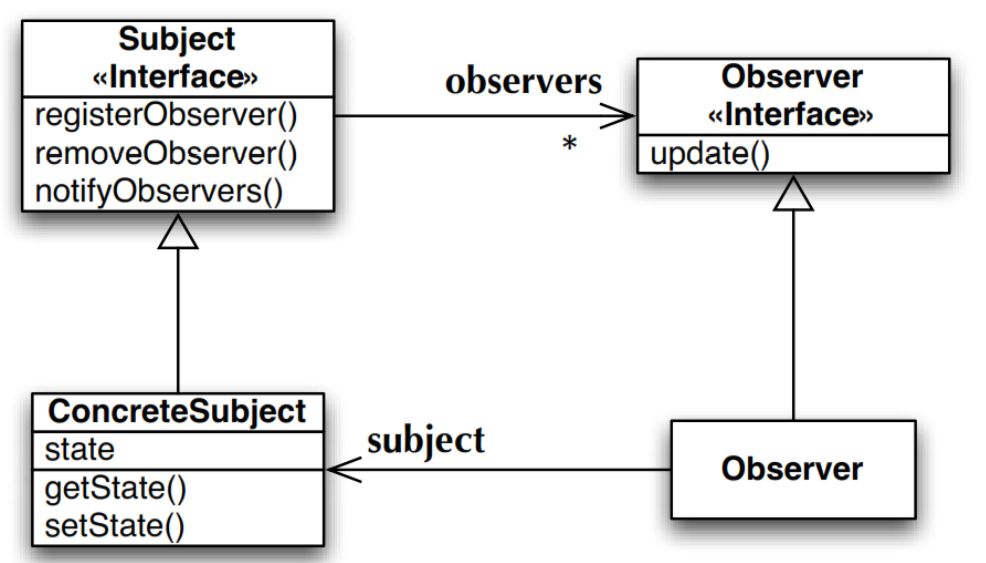
\includegraphics[width=\textwidth]{fig/Observer/structure_observer.png}
    \caption{Mô hình cấu trúc Observer Pattern}
    \label{fig:structure_observer}
\end{figure}
\begin{itemize}
     \item Subject : chứa danh sách các observer,  cung cấp phương thức để có thể thêm và loại bỏ observer.
    \item Observer : định nghĩa một phương thức update() cho các đối tượng sẽ được subject thông báo đến khi có sự thay đổi trạng thái.
    \item ConcreteSubject : cài đặt các phương thức của Subject, lưu trữ trạng thái danh sách các ConcreateObserver, gửi thông báo đến các observer của nó khi có sự thay đổi trạng thái.
    \item ConcreteObserver : cài đặt các phương thức của Observer, lưu trữ trạng thái của subject, thực thi việc cập nhật để giữ cho trạng thái đồng nhất với subject gửi thông báo đến.
\end{itemize}

\section{Cách cài đặt}
\subsection{Cài đặt chung}
Observer tạo ra sự tương tác được kết hợp lỏng lẻo giữa chủ thể và người quan sát
\begin{itemize}
    \item Điều này có nghĩa là họ có thể tương tác với rất ít kiến thức về nhau
\end{itemize} 
Chú ý
\begin{itemize}
    \item đối tượng chỉ biết rằng Observer thực hiện giao diện Observer interface.
    \begin{itemize}
        \item Chúng ta có thể thêm / bớt Observer thuộc bất kỳ loại nào bất kỳ lúc nào.
        \item Chúng ta không bao giờ phải sửa đổi đối tượng để thêm một loại Observer mới.
    \end{itemize}
    \item Chúng ta có thể sử dụng lại đối tượng và Observer trong các trường hợp khác.
    \begin{itemize}
        \item Giao diện plug-and-play ở bất kỳ nơi nào Observer được sử dụng.
    \end{itemize}
    \item Observer có thể phải biết về lớp ConcreteSubject nếu nó cung cấp nhiều phương thức liên quan đến trạng thái khác nhau.
    \begin{itemize}
        \item Mặt khác, dữ liệu có thể được chuyển cho Observer thông qua phương thức update ().
    \end{itemize}
\end{itemize}

Dưới đây là code minh họa cài đặt Observer Pattern.

\begin{figure}[!htb]
    \centering
    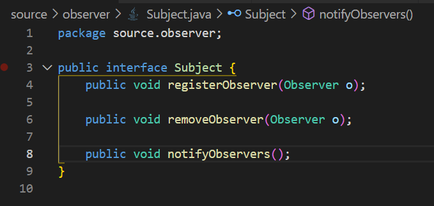
\includegraphics[width=\textwidth]{fig/Observer/subject_class.png}
    \caption{Subject Interface}
    \label{fig:subject_class}
\end{figure}
\begin{figure}[!htb]
    \centering
    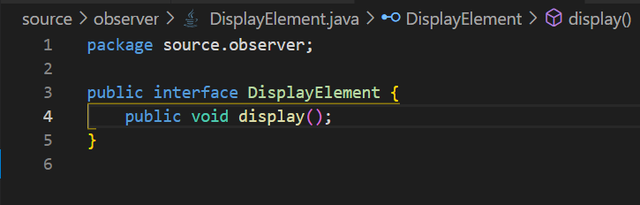
\includegraphics[width=\textwidth]{fig/Observer/display_element_class.png}
    \caption{Display Element Interface}
    \label{fig:display_element_class}
\end{figure}
\newpage
\begin{figure}[!htb]
    \centering
    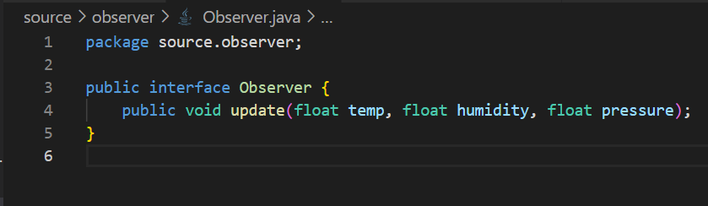
\includegraphics[width=\textwidth]{fig/Observer/observer_class.png}
    \caption{Observer Interface}
    \label{fig:observer_class}
\end{figure}


\subsection{Cài đặt cho một bài toán cụ thể}
Trong bài toán đưa ra ở trên , ta có thể thấy rằng mối quan hệ 1-n ở đây đó là 1-WeatherData và n-Screen . Mỗi khi WeatherData có sự thay đổi về trạng thái (nhiệt độ, độ ẩm, áp suất) thì nó sẽ "thông báo" cho các màn hình đang "quan sát" sát nó để cập nhật lại việc hiển thị thông tin.\\
Do đó chúng ta có Subject ở đây là WeatherData, Observer là các màn hình hiển thị.\\
Mỗi màn hình hiển thị có thể khác nhau, vì thể cách tốt nhất là chúng ta tạo ra một interface cho việc hiển thị.\\
Code minh họa cho bài toán thực tế.\\
Link code cài đặt:
\url{https://github.com/nanhus/OOP-DesginPatten/tree/master/source/observer}
\newpage
\begin{figure}[!htb]
    \centering
    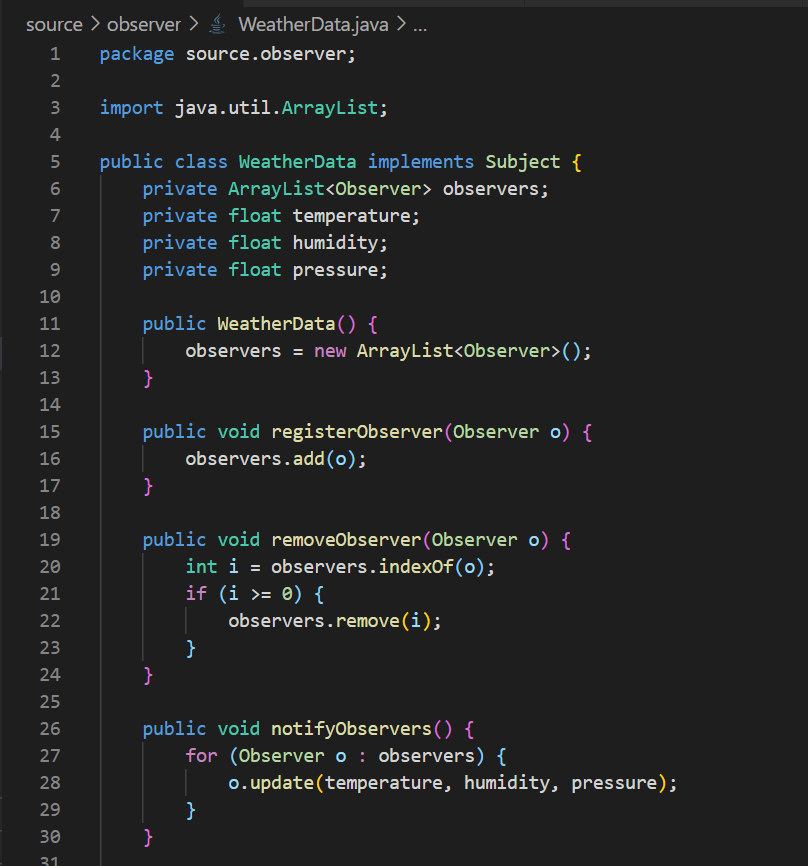
\includegraphics[width=\textwidth]{fig/Observer/weather_data_class.png}
    \caption{Weather Data Class}
    \label{fig:weather_data_class}
\end{figure}
\newpage
\begin{figure}[!htb]
    \centering
    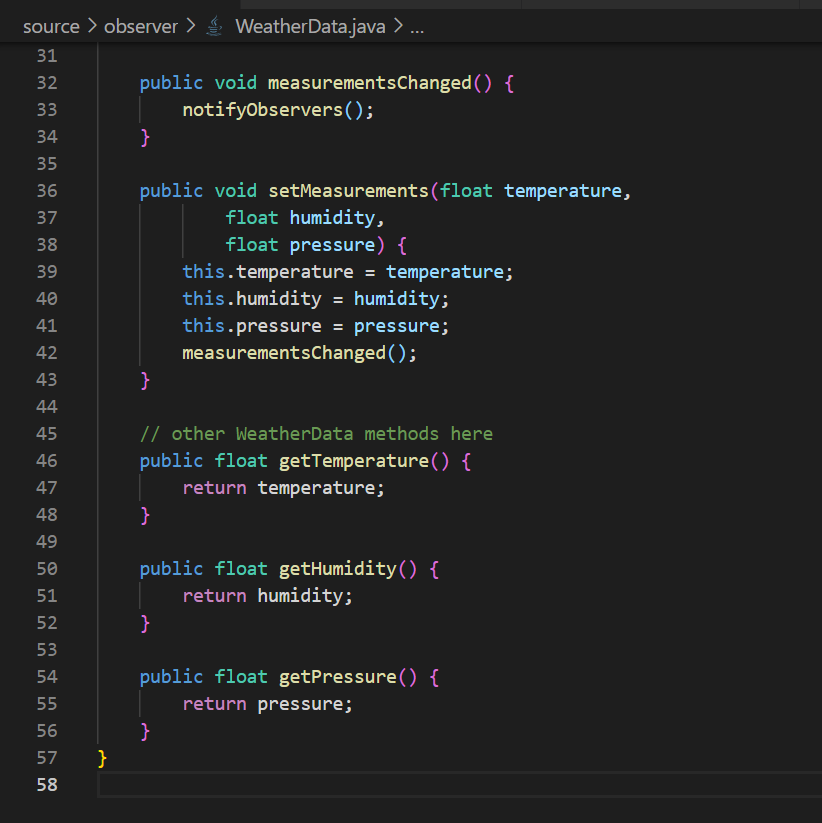
\includegraphics[width=\textwidth]{fig/Observer/weather_data_class_continue.png}
    \caption{Weather Data Class(continue)}
    \label{fig:weather_data_class_continue}
\end{figure}
\newpage
\begin{figure}[!htb]
    \centering
    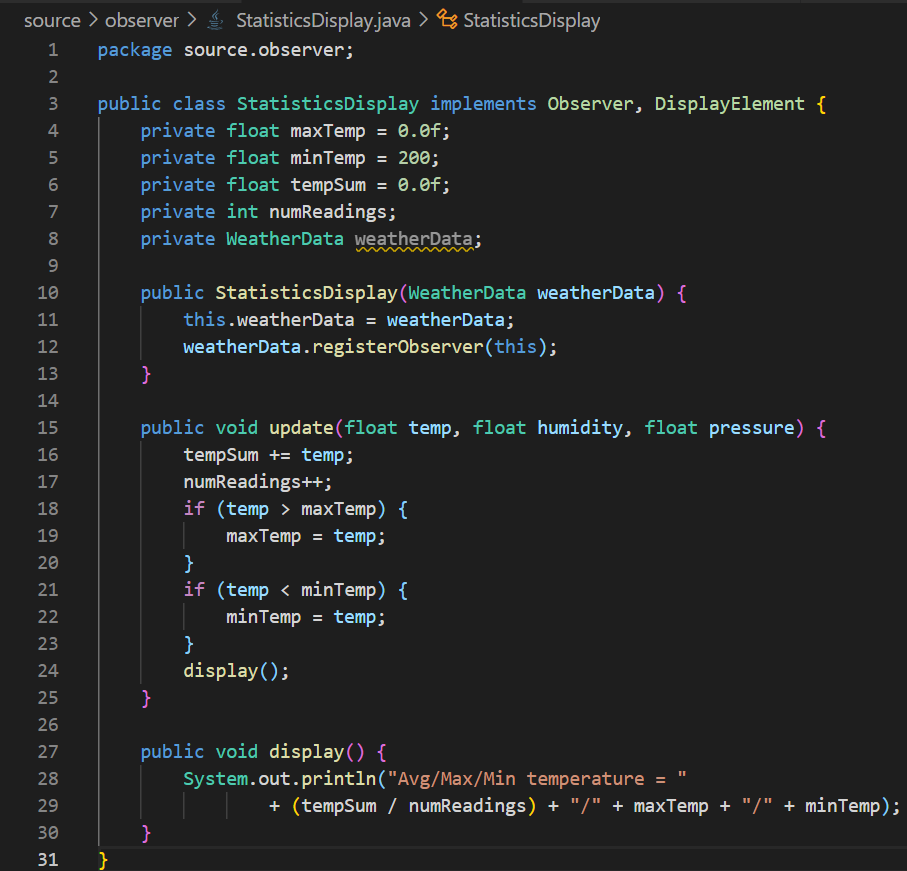
\includegraphics[width=\textwidth]{fig/Observer/statistics_display_class.png}
    \caption{Statistics Display Class}
    \label{fig:statistics_display_class}
\end{figure}
\newpage
\begin{figure}[!htb]
    \centering
    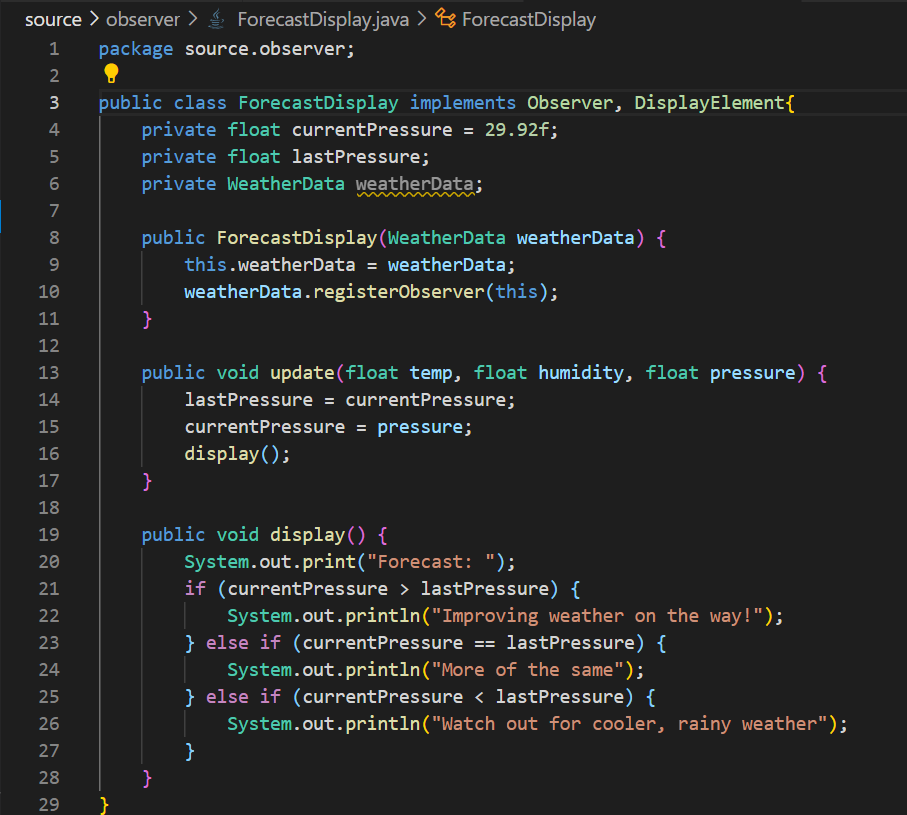
\includegraphics[width=\textwidth]{fig/Observer/forecast_display_class.png}
    \caption{Forecast Display Class}
    \label{fig:forecast_display_class}
\end{figure}
\newpage
\begin{figure}[!htb]
    \centering
    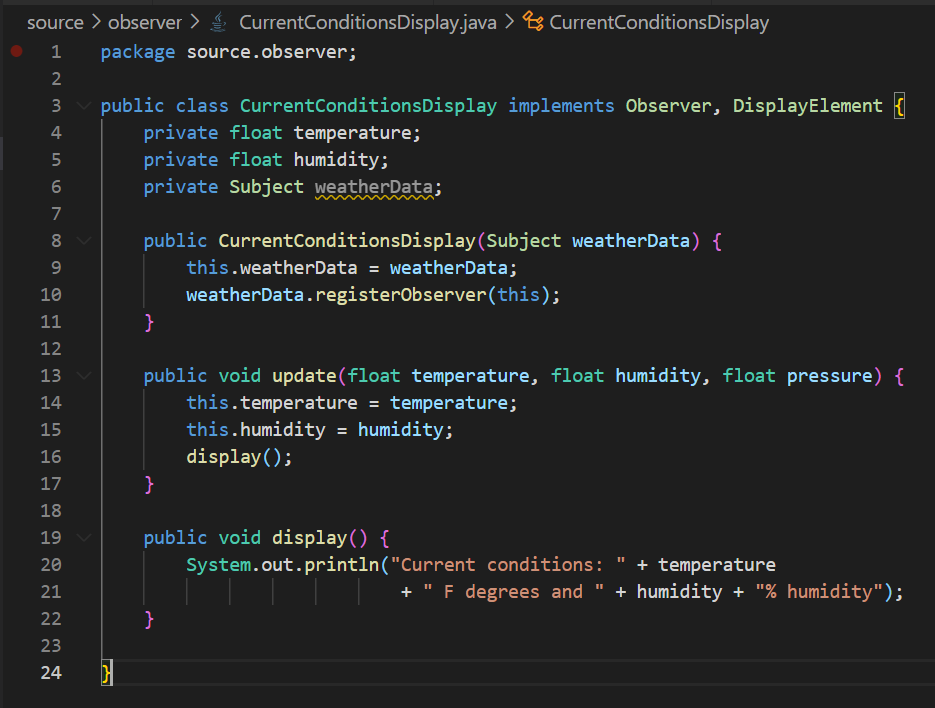
\includegraphics[width=\textwidth]{fig/Observer/current_conditions_display_class.png}
    \caption{Current Conditions Display Class}
    \label{fig:current_conditions_display_class}
\end{figure}
\begin{figure}[!htb]
    \centering
    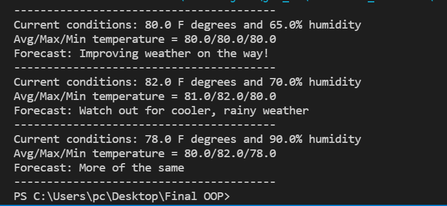
\includegraphics[width=\textwidth]{fig/Observer/observer_output.png}
    \caption{Output}
    \label{fig:observer_output}
\end{figure}

\section{Ví dụ thực tế}
\begin{itemize}
    \item Sử dụng trong ứng dụng broadcast-type communication.
    \item Sử dụng để quản lý sự kiện (Event management).
    \item Sử dụng trong mẫu mô hình MVC (Model View Controller Pattern) : trong MVC, mẫu này được sử dụng để tách Model khỏi View. View đại diện cho Observer và Model là đối tượng Observable.
\end{itemize}
 






\lhead{Design Pattern}
\rhead{State Pattern}
\chapter{6. State Pattern}
\section{Đặt vấn đề - Máy Gumball}
Ngôn ngữ Java đã và đang trở nên rất thịnh hành ở thời điểm hiện tại. Rất nhiều thiết bị hiện đại có thể xây dựng dựa trên Java. Hãy cùng thử làm một chiếc Máy Gumball!\\[0.1in]
Trong máy Gumball có rất nhiều trạng thái được mô tả thông qua lược đồ dưới đây:

\begin{figure}[!htb]
    \centering
    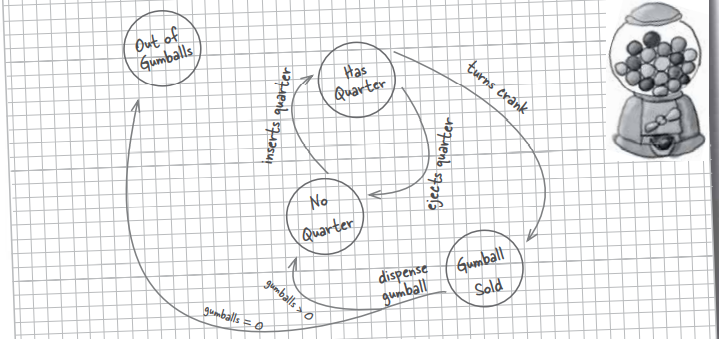
\includegraphics[width=\textwidth]{fig/State/Gumballs_386.png}/
\end{figure}

Bức hình có 4 đường tròn, đó là những trạng thái. \textbf{No Quarter} là trạng thái bắt đầu khi mà trong máy chưa có đồng xu nào. Khi nhét đồng xu vào, nó sẽ chuyển sang trạng thái \textbf{Has Quarter}. Lúc này, ta có thể gạt tay quay để lấy kẹo. Sau đó, máy sẽ kiểm tra lượng kẹo còn lại trong trạng thái \textbf{Gumball Sold} mà quyết định trở về trạng thái \textbf{No Quarter} hay là \textbf{Out of Gumballs}\\[0.1in]

Ta có thể tạo ra lớp \textbf{GumballMachine} như sau:
\begin{itemize}
\item Bước 1: Tập hợp lại các trạng thái:
    \begin{figure}[!htb]
    \centering
    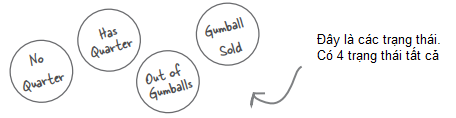
\includegraphics[width=\textwidth]{fig/State/GumballState.png}/
    \end{figure}
\item Bước 2: Tạo các biến static để lưu trạng thái hiện tại và xác định giá trị cho mỗi trạng thái
    \begin{figure}[!htb]
    \centering
    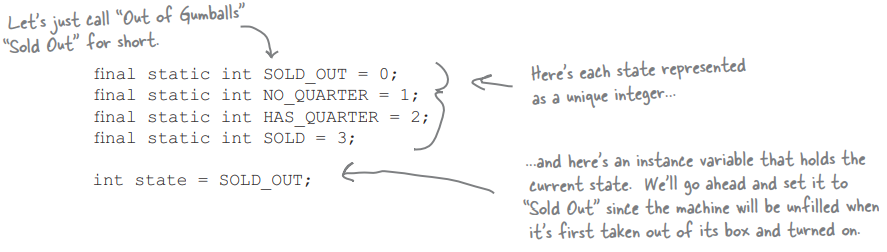
\includegraphics[width=\textwidth]{fig/State/Gumballs_388B2.png}/
    \end{figure}
\item Bước 3: Tập hợp lại những hành động có thể xảy ra trong hệ thống
    \begin{figure}[!htb]
    \centering
    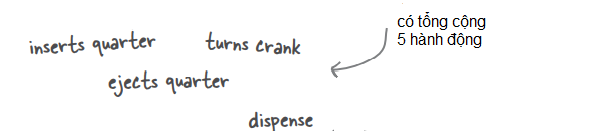
\includegraphics[width=\textwidth]{fig/State/Gumballs_388B3.png}/
    \end{figure}
\item Bước 4: Tạo phương thức ứng với mỗi hành động và sử dụng biểu thức điều kiện để quyết định những hành vi hợp lý ứng với mỗi trạng thái 
\end{itemize}

Dưới đây là code minh họa cho lớp \textbf{GumballMachine}:\newpage

\begin{figure}[!htb]
    \centering
    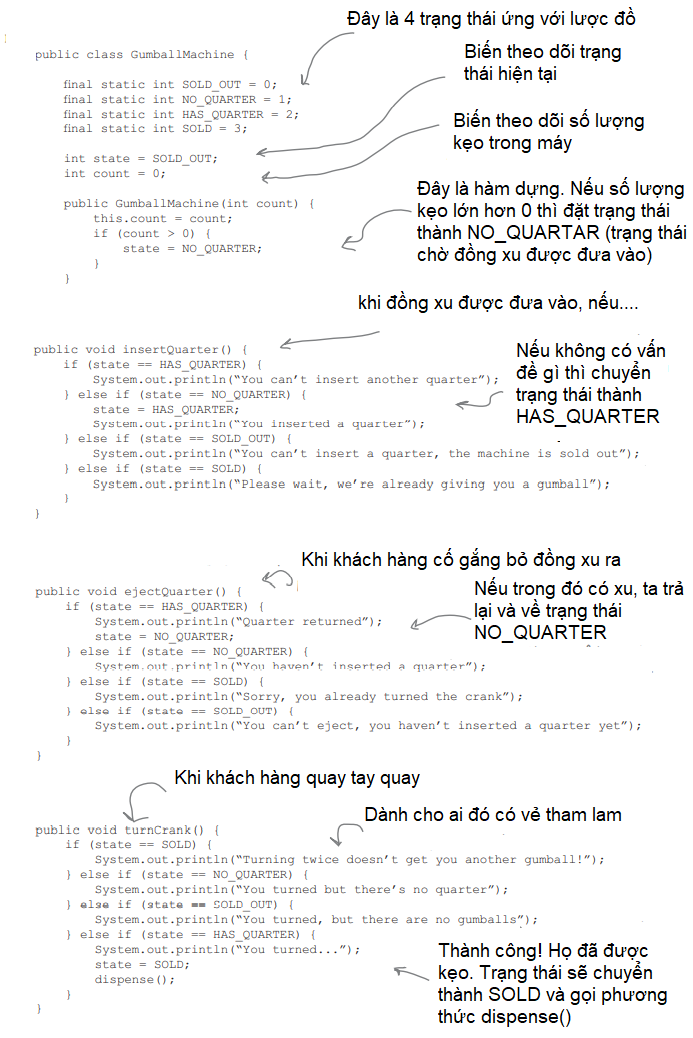
\includegraphics[width=\textwidth]{fig/State/GumballMachine_390.png}/
\end{figure}
\begin{figure}[!htb]
    \centering
    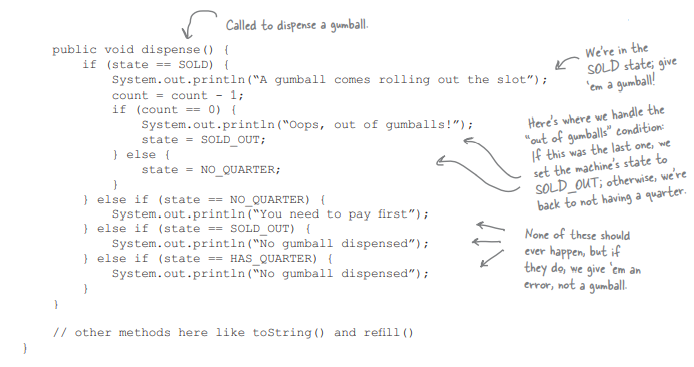
\includegraphics[width=\textwidth]{fig/State/GumballMachine_390_2.png}/
\end{figure}\smallskip

Chương trình ta đã làm rất tuyệt vời nhưng tiếc là đời không như là mơ. Chỉ viết máy Gumball bằng một suy nghĩ thấu đáo như vậy không có nghĩa là nó sẽ dễ dàng phát triển. Giờ khi cải tiến máy với tính năng gấp đôi kẹo nhận được cho người may mắn thì chuyện gì sẽ xảy ra? Khi nghĩ lại đoạn code để nghĩ cách sửa đổi nó thì...
\begin{figure}[!htb]
    \centering
    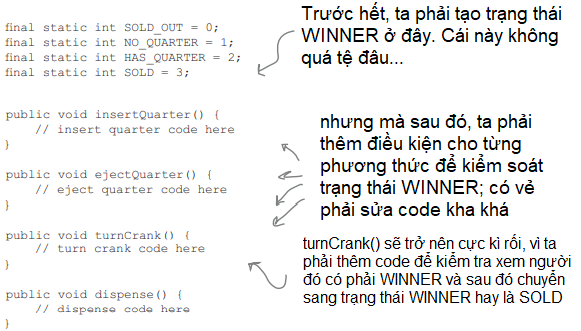
\includegraphics[width=\textwidth]{fig/State/GumballProblem.png}/
\end{figure}\smallskip

\newpage
Vì vấn đề này, ta cần có hướng thiết kế mới. Ta cần cải thiện sao cho code dễ dàng phát triển. Sau đây là cách có thể làm:\smallskip

\begin{itemize}
    \item Trước hết, ta sẽ xác định một \textbf{State Interface} chứa phương thức cho mỗi hành động của máy Gumball
    \item Sau đó, chúng ta bắt đầu cài đặt \textbf{State Class} ứng với mỗi trạng thái của máy. Những lớp này phụ trách cho hành vi của máy khi ở trạng thái tương ứng
    \item Cuối cùng, ta sẽ thay thế biểu thức điều kiện với sự ủy quyền tới những \textbf{State class} để thực hiện công việc
\end{itemize}

Định nghĩa \textbf{State Interface} và các lớp:
\begin{figure}[!htb]
    \centering
    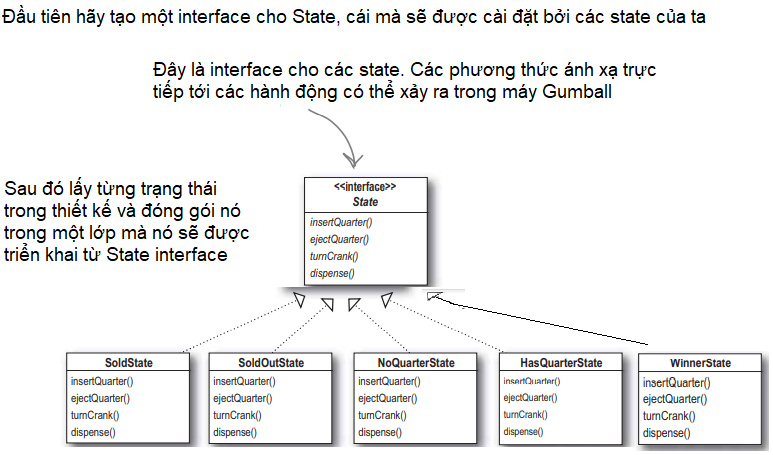
\includegraphics[width=\textwidth]{fig/State/GumballDiagram.png}/
\end{figure}\newpage

Sau đó, tiến hành cài đặt các lớp của \textbf{State}. Bắt đầu với \textbf{NoQuarterState}:
\begin{figure}[!htb]
    \centering
    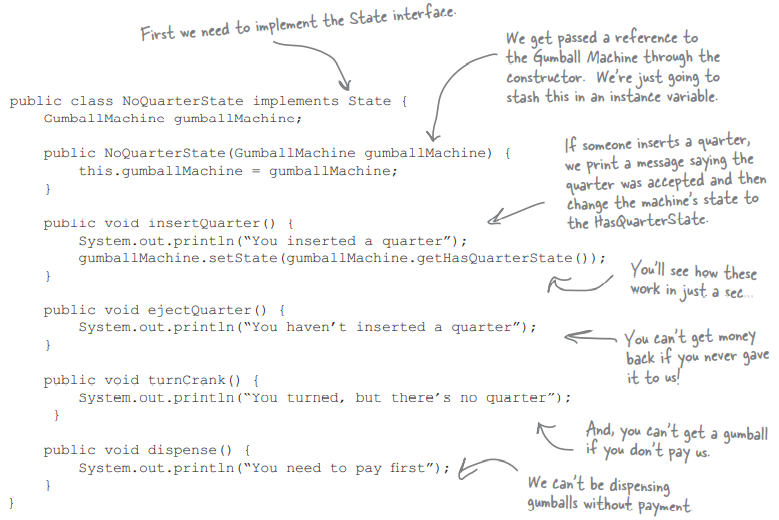
\includegraphics[width=\textwidth]{fig/State/NoQuarterState.png}/
\end{figure}\smallskip

Tiếp theo là \textbf{HasQuarterState} và \textbf{SoldState}:

\begin{figure}[!htb]
    \centering
    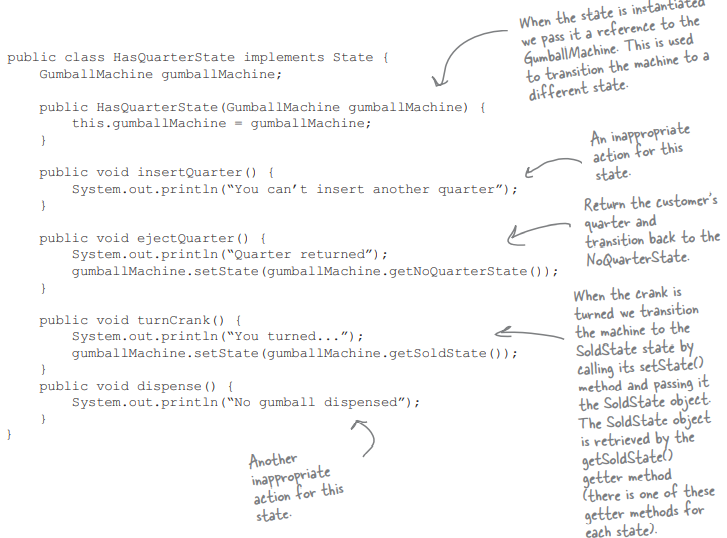
\includegraphics[width=\textwidth]{fig/State/HasQuarterState.png}/
\end{figure}\bigskip

\begin{figure}[!htb]
    \centering
    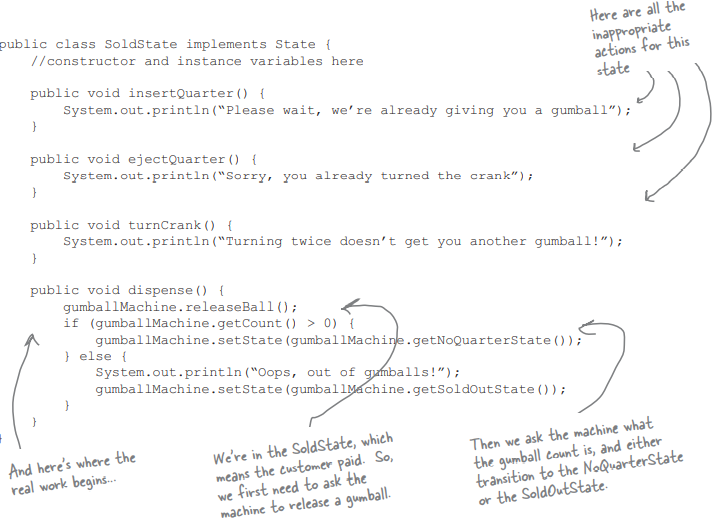
\includegraphics[width=\textwidth]{fig/State/SoldState.png}/
\end{figure}\newpage

Tương tự với 2 \textbf{SoldOutState} và \textbf{WinnerState}. Cuối cùng là lóp \textbf{GumballMachine} hoàn chỉnh:

\begin{figure}[!htb]
    \centering
    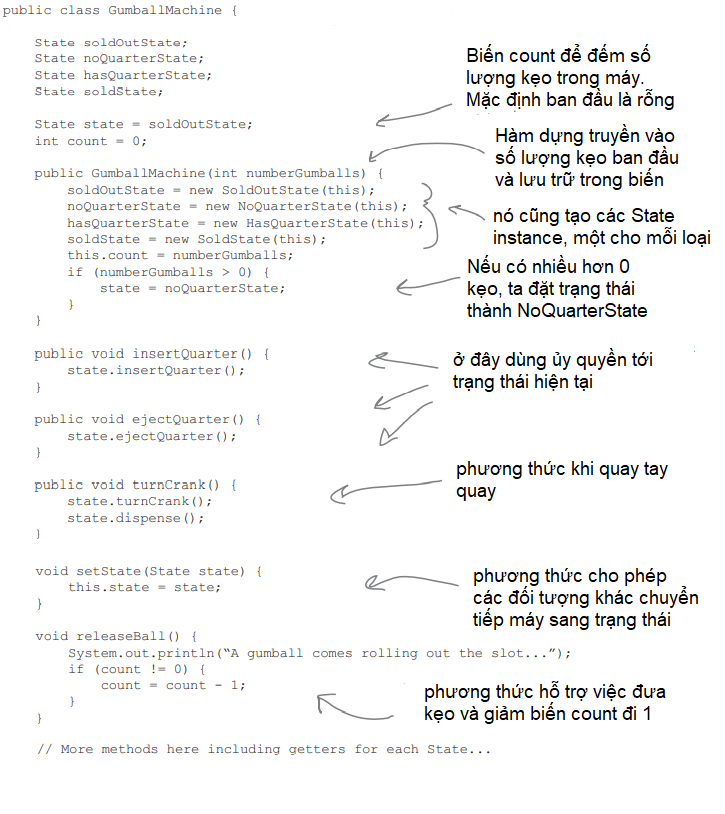
\includegraphics[width=\textwidth]{fig/State/GumballMachine_code.png}/
\end{figure}

Nhìn lại những gì trước đó đã làm, ta đã thay đổi cấu trúc khác biệt so với bản đầu tiên nhưng chức năng vẫn không đổi. Cách thiết kế này có tên gọi là \textbf{State Pattern} Bằng cách này, ta đã:

\begin{itemize}
    \item Tách biệt hành vi của từng trạng thái đến từng lớp
    \item Loại bỏ tất cả biểu thức điều kiện rắc rối gây khó khăn trong việc bảo trì
    \item Đóng từng trạng thái cho việc sửa đổi nhưng vẫn để Máy Gumball được phát triển bằng cách thêm mới nhiều lớp trạng thái
    \item Tạo một code base và cấu trúc lớp ánh xạ tương đồng tới bản thiết kế ban đầu, dễ đọc, dễ hiểu
\end{itemize}

\section{Định nghĩa và Mô hình cấu trúc}
\subsection{Định nghĩa}
\textbf{State Pattern} cho phép một đối tượng thay đổi hành vi của nó khi trạng thái bên trong thay đổi. Đối tượng sẽ xuất hiện để thay đổi lớp của nó
\subsection{Mô hình cấu trúc}
Dưới đây là mô hình cấu trúc của \textbf{State Pattern}:
\begin{figure}[!htb]
    \centering
    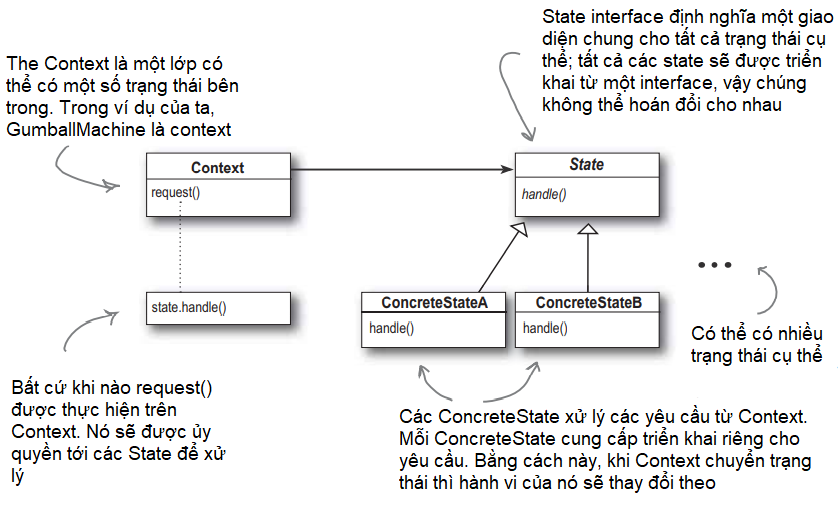
\includegraphics[width=\textwidth]{fig/State/StateDiagram.png}/
\end{figure}

\section{Thực tế}
Johnson and Zweig [JZ91] biểu thị State pattern và ứng dụng tới giao thức kết nối TCP\\[0.1in]
Hầu hết các chương trình vẽ phổ biến đều cung cấp "công cụ" để thực hiện các thao tác trực tiếp. Ví dụ: một công cụ vẽ đoạn thẳng cho phép người dùng nhấp và kéo để tạo một đường mới. Một công cụ lựa chọn cho phép người dùng chọn các hình khối. Thường có một bảng các công cụ để lựa chọn. Người dùng coi việc này này như nhặt một dụng cụ và sử dụng nó, nhưng trên thực tế, hành vi của editor thay đổi với công cụ hiện tại: Khi một công cụ vẽ hoạt động, ta tạo ra các hình khối; khi mà
công cụ lựa chọn đang hoạt động ,ta chọn các hình khối đó; và cứ thế. Ta sử dụng State pattern để thay đổi hành vi của editor tùy thuộc vào công cụ hiện tại.\\[0.1in]
Ta có thể định nghĩa lớp trừu tượng Tool để từ đó định nghĩa các lớp con mà cài đặt các hành vi cụ thể. Trình chỉnh sửa bản vẽ duy trì một đối tượng Tool và ủy quyền các yêu cầu tới nó. Trình sẽ thay thế đối tượng khi người dùng chọn công cụ mới khiến hành vi của trình vẽ thay đổi theo\\[0.1in]
Kĩ thuật này được áp dụng dụng trong những framework hỗ trợ chỉnh sửa bản vẽ điển hình như HotDraw [Joh92] và Unidraw [VL90]. Nó cho phép phía Client định nghĩa nhiều loại công cụ một cách dễ dàng. Trong HotDraw, lớp DrawingController chuyển tiếp các yêu cầu đến đối tượng Tool hiện tại. Còn Unidraw sẽ có lớp tương ứng là Viewer và Tool. Dưới đây là mô hình cấu trúc cho Tool và DrawingController interfaces:
\begin{figure}[!htb]
    \centering
    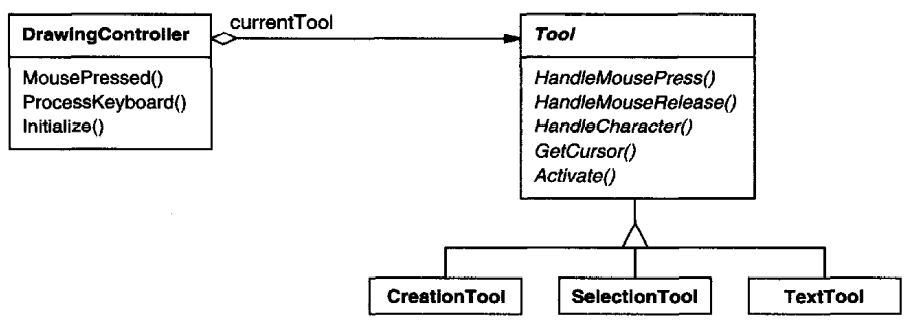
\includegraphics[width=\textwidth]{fig/State/StateRealLifeEX.png}/
\end{figure}

\lhead{Design Pattern}
\rhead{Factory Pattern}
\chapter{7. Factory Pattern}
\section{Giới thiệu}
\subsection{Đặt vấn đề}
Vấn đề.
\begin{itemize}
    \item Làm thế nào một ứng dụng có thể độc lập với cách các đối tượng của nó được tạo ra?
    \item Làm thế nào một lớp có thể độc lập với cách các đối tượng mà nó yêu cầu được tạo ra?
    \item Làm thế nào có thể tạo mối quan hệ của các đối tượng liên quan hoặc phụ thuộc?
\end{itemize}
Việc tạo các đối tượng trực tiếp bên trong lớp yêu cầu các đối tượng là không linh hoạt vì nó gán lớp với các đối tượng cụ thể và khiến nó không thể thay đổi việc khởi tạo sau này một cách độc lập với (mà không cần phải thay đổi) lớp. Nó ngăn lớp không thể sử dụng lại nếu các đối tượng khác được yêu cầu và nó làm cho lớp khó kiểm tra vì không thể thay thế các đối tượng thực bằng các đối tượng giả.\\
Factory Pattern mô tả cách giải quyết các vấn đề như vậy.

\subsection{Mục đích sử dụng}
Mục đích sử dụng:
\begin{itemize}
    \item Giúp việc khởi tạo các đối tượngs mà che giấu đi xử lí logic của việc khởi tạo đó. Người dùng không biết logic thực sự được khởi tạo bên dưới phương thức factory.
    \item Mẫu thiết kế này cho phép các lớp con chọn kiểu đối tượng cần tạo.
    \item Nó thúc đẩy sự liên kết lỏng lẻo bằng cách loại bỏ sự cần thiết phải ràng buộc các lớp cụ thể vào code. Nghĩa là code chỉ tương tác với interface hoặc lớp abstract, để nó sẽ làm việc với bất kỳ lớp nào implements interface đó hoặc extends lớp abstract.
    \item Factory Pattern giúp giảm sự phụ thuộc giữa các module: cung cấp 1 hướng tiếp cận với Interface thay vì các implement. Giúp chuơng trình độc lập với những lớp cụ thể mà chúng ta cần tạo 1 đối tượng, code ở phía client sẽ không bị ảnh hưởng khi thay đổi logic ở factory hay sub class.
    \item Việc mở rộng code dễ dàng hơn: khi cần mở rộng, chỉ việc tạo ra những sub class và implement thêm vào factory method.
    \item Dễ dạng quản lý life cycle của các đối tượng được tạo bởi Factory Method Pattern.
    \item Thống nhất về mặt naming convention: giúp cho các developer có thể hiểu về cấu trúc source code.
\end{itemize}

\section{Định nghĩa và mô hình cấu trúc}
\subsection{Định nghĩa}
Mẫu thiết kế Factory Method xác định một giao diện để tạo một đối tượng, nhưng cho phép các lớp con
quyết định lớp sẽ khởi tạo. Factory Method cho phép một class trì hoãn việc khởi tạo thành các lớp subclass.
Mẫu thiết kế Abstract Factory cung cấp một giao diện để tạo các họ có liên quan hoặc các đối tượng phụ thuộc mà không chỉ định các lớp cụ thể của chúng
\subsection{Mô hình cấu trúc}
\begin{figure}[!htb]
    \centering
    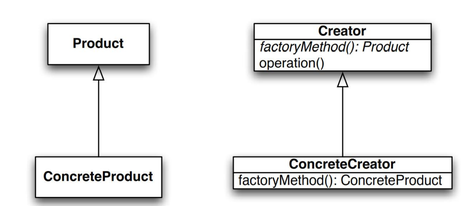
\includegraphics[width=\textwidth]{fig/Factory/structure_factory_method.png}
    \caption{Mô hình cấu trúc Factory Method}
    \label{fig:structure_factory_method}
\end{figure}
\begin{figure}[!htb]
    \centering
    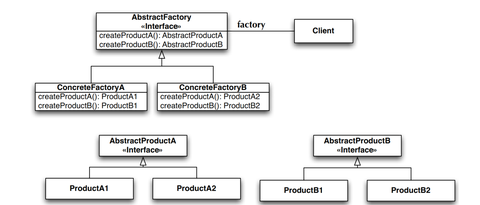
\includegraphics[width=\textwidth]{fig/Factory/structure_factory.png}
    \caption{Mô hình cấu trúc Factory Pattern}
    \label{fig:structure_factory}
\end{figure}
\begin{itemize}
    \item Super Class: môt supper class trong Factory Pattern có thể là một interface, abstract class hay một class thông thường.
    \item Sub Classes: các sub class sẽ cài đặt các phương thức của supper class theo nghiệp vụ riêng của nó.
    \item Factory Class: một class chịu tránh nhiệm khởi tạo các đối tượng sub class dựa theo tham số đầu vào. Lưu ý: lớp này là Singleton hoặc cung cấp một public static method cho việc truy xuất và khởi tạo đối tượng. Factory class sử dụng if-else hoặc switch-case để xác định class con đầu ra.
\end{itemize}
\section{Cách cài đặt}
Cài đặt Factory Pattern qua 1 bài toán thực tế theo sơ đồ dưới đây.

\begin{figure}[!htb]
    \centering
    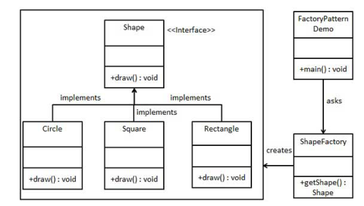
\includegraphics[width=\textwidth]{fig/Factory/example_structure_factory.png}
    \caption{Mô hình ví dụ}
    \label{fig:example_structure_factory}
\end{figure}
Cách cài đặt.
\\Link code cài đặt:
\url{https://github.com/nanhus/OOP-DesginPatten/tree/master/source/factory}\\

Bước 1: Tạo 1 giao diện.
\begin{figure}[!htb]
    \centering
    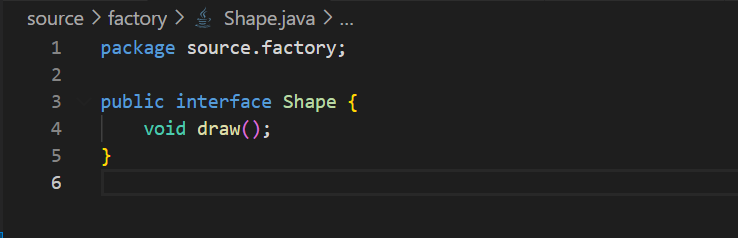
\includegraphics[width=\textwidth]{fig/Factory/shape_class.png}
    \caption{Shape interface}
    \label{fig:shape_class}
\end{figure}

\newpage
Bước 2: Tạo các đối tượng cụ thể cài đặt giao diện Shape.
\begin{figure}[!htb]
    \centering
    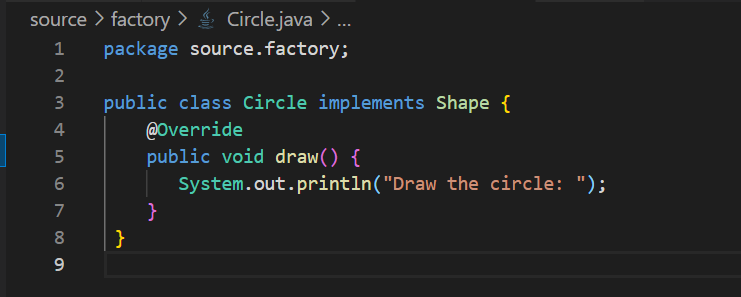
\includegraphics[width=\textwidth]{fig/Factory/circle_class.png}
    \caption{Circle Class}
    \label{fig:circle_class}
\end{figure}

\begin{figure}[!htb]
    \centering
    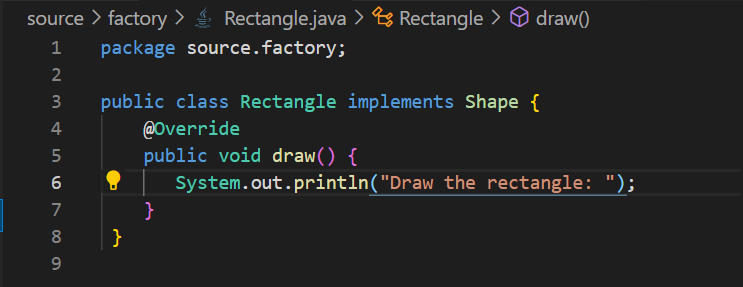
\includegraphics[width=\textwidth]{fig/Factory/rectangle_class.png}
    \caption{Rectangle Class}
    \label{fig:rectangle_class}
\end{figure}

\begin{figure}[!htb]
    \centering
    \includegraphics[width=\textwidth]{fig/Factory/square_class.png}
    \caption{Square Class}
    \label{fig:square_class}
\end{figure}

\newpage
Bước 3:Tạo một class ShapeFactory để tạo đối tượng của lớp cụ thể dựa trên thông tin đã cho.

\begin{figure}[!htb]
    \centering
    \includegraphics[width=\textwidth]{fig/Factory/shape_factory_class.png}
    \caption{Shape Factory Class}
    \label{fig:shape_factory_class}
\end{figure}

Bước 4:Sử dụng Factory để lấy đối tượng của lớp cụ thể bằng cách truyền một thông tin như kiểu.

\begin{figure}[!htb]
    \centering
    \includegraphics[width=\textwidth]{fig/Factory/demo_factory_class.png}
    \caption{Demo Factory class}
    \label{fig:demo_factory_class}
\end{figure}

\newpage
Output:
\begin{figure}[!htb]
    \centering
    \includegraphics[width=\textwidth]{fig/Factory/factory_output.png}
    \caption{Output}
    \label{fig:factory_output}
\end{figure}

\section{Ví dụ thực tế}
\begin{itemize}
    \item Áp dụng quản lí các mặt hàng
    \item JDK: java.util.Calendar, ResourceBundle, NumberFormat, …
    \item BeanFactory trong Spring Framework.
    \item SessionFactory trong Hibernate Framework.
    \item Nó định nghĩa các Abstract Factory trong WidgetKit và DialogKit để tạo ra các đối tượng giao diện người dùng có giao diện cụ thể.
    \item Sử dụng mẫuAbstract Factory để đạt được tính di động trên các hệ thống khác nhau (ví dụ: X Windows và SunView). Lớp trừu tượng WindowSystem xác định giao diện để tạo đối tượng đại diện cho tài nguyên hệ thống cửa sổ (ví dụ: MakeWindow, MakeFont, MakeColor).
\end{itemize}



\lhead{Design Pattern}
\rhead{Composite Pattern}
\chapter{8. Composite Pattern}
\section{Giới thiệu tổng quan}

Nhắc đến cụm từ \textbf{Composite} thì \textbf{Composite} được hiểu như một thứ được tạo nên từ các thành phần. Một \textbf{Đối tượng Composite} là một đối tượng được tạo nên bởi nhiều đối tượng. Ví dụ như một chiếc ô tô được tạo nên bởi 4 chiếc bánh xe vậy hay nước được tạo bởi Hydro và Oxy vậy. Đó là cách mà \textbf{Composite Pattern} được tạo ra. Xét những trường hợp mà ta muốn gom một nhóm đối tượng thành một tập hợp để thuận tiện trong quá trình thao tác

\section{Định nghĩa và Mô hình cấu trúc}
\subsection{Định nghĩa}
\textbf{Composite Pattern} cho phép ta tổ chức những đối tượng dưới dạng cây phân tầng. \textbf{Composite} cho phép coi các đối tượng riêng lẻ và các thành phần của các đối tượng như một thể thống nhất

\begin{figure}[!htb]
    \centering
    \includegraphics[width=\textwidth]{fig/Composite/CompositeStructure.png}/
\end{figure}
\newpage
\subsection{Mô hình cấu trúc}
Mô hình cấu trúc của \textbf{Composite Pattern} được biểu diễn như sau:

\begin{figure}[!htb]
    \centering
    \includegraphics[width=\textwidth]{fig/Composite/CompositeDiagram.png}/
\end{figure}

\begin{itemize}
    \item \textbf{Base Component}: Là một \textbf{Interface} hoặc \textbf{Abstract Class} quy định các phương thức chung cần phải có cho tất cả các thành phần tham gia
    \item \textbf{Leaf}: Là lớp thực hiện cài đặt phương thức của \textbf{Component} và không chứa lớp con
    \item \textbf{Composite}: Là lớp có vai trò lưu trữ và thao tác tập hợp các \textbf{Leaf}
    \item \textbf{Client}: Là nơi sử dụng \textbf{Base Component} để làm việc với các đối tượng trong \textbf{Composition}
\end{itemize}\smallskip

\textbf{Lưu ý}: Một \textbf{composite} chứa các \textbf{component} vì \textbf{component} có thể là \textbf{composite} hoặc \textbf{leaf}. Nghe vẻ có mùi đệ quy ở đây nhỉ? Có vẻ là vậy vì một \textbf{composite} chứa tập hợp các nút con, những nút con có thể là \textbf{composite} hoặc \textbf{leaf}\newpage

\section{Ví dụ}

Để hiểu hơn Composite Pattern, xét ví dụ về bài toán quản lý tệp tin:

\begin{figure}[!htb]
    \centering
    \includegraphics[width=\textwidth]{fig/Composite/FileStructure.png}/
\end{figure}

Một hệ thống tệp tin là hệ thống có cấu trúc cây phân cấp trong đó có các File và Folder. Một Folder có thể chứa nhiều File và Folder bên trong nên ta có thể coi Folder như \textbf{Composite} còn File sẽ là \textbf{Leaf}. Ta có mô hình cấu trúc ở bên dưới:

\begin{figure}[!htb]
    \centering
    \includegraphics[width=\textwidth]{fig/Composite/FileDiagram.png}/
\end{figure}\newpage

Đầu tiên ta định nghĩa cho \textbf{component} Interface có các phương thức chung cho cả File và Folder. Để đơn giản, ví dụ này chỉ bảo gồm 2 phương thức \textbf{showProperty()} và \textbf{totalSize()}. Hai phương thức này sẽ lấy ra thông tin của File/Folder và tổng kích thước của chúng

\begin{figure}[!htb]
    \centering
    \includegraphics[width=\textwidth]{fig/Composite/FileComponent.png}/
\end{figure}

Tiếp theo, ta tạo lớp \textbf{Leaf} cài đặt các phương thức của \textbf{component}, gọi là \textbf{FileLeaf}. Sau đó tạo lớp \textbf{Composite} chứa tập hợp các \textbf{Leaf} và cài đặt các phương thức của lớp \textbf{component}, gọi là \textbf{FolderComposite}\\[0.1in]

Lớp \textbf{FileLeaf}:
\begin{figure}[!htb]
    \centering
    \includegraphics[width=\textwidth]{fig/Composite/FileLeaf.png}/
\end{figure}\newpage

Lớp \textbf{FolderComposite}:
\begin{figure}[!htb]
    \centering
    \includegraphics[width=\textwidth]{fig/Composite/FolderComposite.png}/
\end{figure}

Cuối cùng, ta hoàn thiện lớp \textbf{Client} để chạy chương trình:
\begin{figure}[!htb]
    \centering
    \includegraphics[width=\textwidth]{fig/Composite/FileClient.png}/
\end{figure}\newpage

Output của chương trình:
\begin{figure}[!htb]
    \centering
    \includegraphics[width=\textwidth]{fig/Composite/FileOutput.png}/
\end{figure}

\section{Thực tế}
\textbf{Composite Pattern} có thể được tìm thấy tại hầu hết các hệ thống lập trình theo hướng đối tượng. Lớp Viewer gốc của Smalltalk Model/View/Controller [KP88] là \textbf{Composite}, và gần như bộ giao diện người dùng và framework. Viewer thời điểm đó vừa là lớp \textbf{Component} vừa là lớp \textbf{Composite}. Bản 4.0 của Smalltalk-80 sửa lại Model/View/Controller với một lớp VisualComponent có những lớp con là View và CompositeView\\[0.1in]
RTL Smalltalk compiler framework sử dụng Composite Pattern một cách chuyên sâu. RTLExpression là một lớp \textbf{Component} cho cây phân tích cú pháp. Nó có những lớp con như BinaryExpression chứa những đối tượng RTLExpression. Những lớp này định nghĩa một cấu trúc composite cho cây phân tích cú pháp. RegisterTransfer là một lớp \textbf{Component} cho chương trình trung gian Single Static Assignment (SSA). Những lớp con Leaf của RegisterTransfer xác định các nhiệm vụ tĩnh khác nhau\\[0.1in]
Một ví dụ khác cho pattern này xảy ra trong lĩnh vực tài chính, nơi mà có một danh mục đầu tư tổng hợp các tài sản riêng lẻ. 
Ta có thể hỗ trợ các tổng hợp phức tạp của tài sản bằng cách cài đặt "danh mục đầu tư" như một lớp \textbf{Composite} phù hợp với giao diện của một tài sản cá nhân [BE93].

\lhead{Design Pattern}
\rhead{Iterator Pattern}
\chapter{9. Iterator}
\section{Giới thiệu}
\subsection{Đặt vấn đề}
Trong khi phát triển các ứng dụng, chúng ta làm việc với nhiều loại cấu trúc dữ liệu như: cấu trúc cây, mảng, tập hợp, bảng băm, ngăn xếp, hàng đợi, … Cách thức mà các cấu trúc dữ liệu này lưu trữ đối tượng của nó rất khác nhau, và nếu bạn muốn truy cập dữ liệu của những đối tượng này, bạn phải học những kỹ thuật khác nhau cho từng loại cấu trúc dữ liệu. Khi đó, mẫu Iterator là một giải pháp tốt.\\
Chúng ta có thể sử dụng một interface được xác định phương thức cụ thể để truy cập tới từng phần tử của cấu trúc dữ liệu. Sử dụng những phương thức này, chúng ta có thể truy xuất tới các phần tử trong tập hợp theo cùng cách dễ dàng nhất.

\begin{figure}[!htb]
    \centering
    \includegraphics[width=\textwidth]{fig/Iterator/iterator_problem.png}
    \caption{Các loại tập hợp}
    \label{fig:iterator_problem}
\end{figure}

\subsection{Mục đích sử dụng}
\begin{itemize}
    \item Đảm bảo nguyên tắc Single responsibility principle (SRP) : chúng ta có thể tách phần cài đặt các phương thức của tập hợp và phần duyệt qua các phần tử (iterator) theo từng class riêng lẻ.
    \item Đảm bảo nguyên tắc Open/Closed Principle (OCP) : chúng ta có thể implement các loại collection mới và iterator mới, sau đó chuyển chúng vào code hiện có mà không vi phạm bất cứ nguyên tắc gì.
    \item Chúng ta có thể truy cập song song trên cùng một tập hợp vì mỗi đối tượng iterator có chứa trạng thái riêng của nó.
\end{itemize}

\section{Định nghĩa và Mô hình cấu trúc}
\subsection{Định nghĩa}
Iterator Pattern là một trong những Pattern thuộc nhóm hành vi (Behavioral). Nó được sử dụng để cung cấp một cách thức truy cập tuần tự tới các phần tử của một đối tượng tổng hợp, mà không cần phải tạo dựng riêng các phương pháp truy cập cho đối tượng tổng hợp này.

\subsection{Mô hình cấu trúc}
\begin{figure}[!htb]
    \centering
    \includegraphics[width=\textwidth]{fig/Iterator/structure_iterator.png}
    \caption{Mô hình cấu trúc}
    \label{fig:structure_iterator}
\end{figure}

\begin{itemize}
    \item Aggregate : là một interface định nghĩa các phương thức để tạo Iterator object.
    \item ConcreteAggregate : cài đặt các phương thức của Aggregate, nó cài đặt interface tạo Iterator để trả về một thể hiện của ConcreteIterator thích hợp.
    \item Iterator : là một interface hay abstract class, định nghĩa các phương thức để truy cập và duyệt qua các phần tử.
    \item ConcreteIterator : cài đặt các phương thức của Iterator, giữ index khi duyệt qua các phần tử.
    \item Client : đối tượng sử dụng Iterator Pattern, nó yêu cầu một iterator từ một đối tượng collection để duyệt qua các phần tử mà nó giữ. Các phương thức của iterator được sử dụng để truy xuất các phần tử từ collection theo một trình tự thích hợp
\end{itemize}

\section{Cách cài đặt}
Cài đặt Iterator để duyệt qua các item trong một menu.\\
Link code cài đặt:
\url{https://github.com/nanhus/OOP-DesginPatten/tree/master/source/iterator}
\begin{figure}[!htb]
    \centering
    \includegraphics[width=\textwidth]{fig/Iterator/iterator_example.png}
    \caption{Mô hình cấu trúc}
    \label{fig:iterator_example}
\end{figure}
Dưới đây là code minh họa cài đặt:
\begin{figure}[!htb]
    \centering
    \includegraphics[width=\textwidth]{fig/Iterator/item_class.png}
    \caption{Item Class}
    \label{fig:item_class}
\end{figure}
\begin{figure}[!htb]
    \centering
    \includegraphics[width=\textwidth]{fig/Iterator/item_iterator_interface.png}
    \caption{Item Iterator Interface}
    \label{fig:item_iterator_interface}
\end{figure}
\begin{figure}[!htb]
    \centering
    \includegraphics[width=\textwidth]{fig/Iterator/menu_class.png}
    \caption{Menu Class}
    \label{fig:menu_class}
\end{figure}
\begin{figure}[!htb]
    \centering
    \includegraphics[width=\textwidth]{fig/Iterator/client_class.png}
    \caption{Client Class}
    \label{fig:client_class}
\end{figure}
\begin{figure}
    \centering
    \includegraphics[width=\textwidth]{fig/Iterator/iterator_output.png}
    \caption{Output}
    \label{fig:iterator_output}
\end{figure}

\newpage
\section{Ví dụ thực tế}
\begin{itemize}
    \item Truy xuất nhiều loại tập hợp
    \item Ứng dụng trong chuyển kênh của vô tuyến tuyền hình
    \item Ví dụ trong thư viện java
    \begin{itemize}
        \item java.util.Iterator 
        \item java.util.Enumeration
    \end{itemize}
    \item ObjectWindows 2.0 [Bor94] cung cấp một lớp phân cấp những iterator cho các container. Ta có thể duyệt các container khác nhau bằng việc sử dụng toán tử ++ để đưa iterator đến vị trí kế tiếp
\end{itemize}




\lhead{Design Pattern}
\rhead{Builder Pattern}
\chapter{10. Builder Pattern}
\section{Đặt vấn đề}
Ta chắc hẳn đã biết về lợi ích to lớn mà \textbf{immutability} và immutale instances trong ứng dụng. Chưa được thuyết phục lắm? Vậy hãy nhìn lại về lớp \textbf{String} trong Java tại \href{https://howtodoinjava.com/java/string/java-interview-question-why-strings-are-immutable/}{\textbf{đây}}\\[0.1in]
Hãy bàn luận một chút về vấn đề trong ứng dụng của chúng ta. Trong bất kì module quản lý người dùng nào, thực thể chính luôn là người dùng. Một khi người dùng được tạo ra thì ta không muốn thay đổi trạng thái của nó. Điều này có vẻ mâu thuẫn nhỉ...\\[0.1in]
Bây giờ, hãy giả sử, đối tượng người dùng của ta có 5 thuộc tính: Họ, tên, tuổi, số điện thoại và địa chỉ\\[0.1in]
Thông thường, khi ta thiết kế lớp người dùng, ta phải truyền tất cả tham số vào hàm dựng như sau:\\[0.1in]
\begin{figure}[!htb]
    \centering
    \includegraphics[width=\textwidth]{fig/Builder/UserNormalDesign.png}
\end{figure}\\[0.1in]
Vậy chuyện gì xảy ra nếu ta không bắt buộc 3 trường tuổi, số điện thoại và địa chỉ? Khi đó sẽ xảy ra vấn đề. Ta cần nhiều hàm dựng hơn và dẫn đến tình trạng \textbf{telescoping constructors}. Nói cách khác, cách thiết kế này sẽ mất tính thẩm mĩ và rất là rối
\begin{figure}[!htb]
    \centering
    \includegraphics[width=\textwidth]{fig/Builder/UglyDesign.png}
\end{figure}\\[0.1in]
\textbf{Builder Pattern} sinh ra để khắc phục vấn đề này. Nó giúp ta có thể tạo lớp immutable kiểm soát một đối tượng phức tạp có số lượng thuộc tính đủ lớn
\section{Định nghĩa và Mô hình cấu trúc}
\subsection{Định nghĩa}
\textbf{Builder Pattern} là một pattern tách biệt cách dựng của một đối tượng phức tạp khỏi sản phầm cuối cùng. Bằng cách này, cùng một cách dựng có thể tạo ra nhiều sản phẩm khác nhau. Cũng như \textbf{Factory Pattern}, \textbf{Builder Pattern} thuộc nhóm \textbf{Creational Pattern} (Nhóm khởi tạo)
\section{Mô hình cấu trúc}
Mô hình cấu trúc của Builder Pattern được mô tả như sau:
\begin{figure}[!htb]
    \centering
    \includegraphics[width=\textwidth]{fig/Builder/BuilderDiagram.png}
    \caption{Mô hình cấu trúc Builder Pattern}
\end{figure}
Trong đó:
\begin{itemize}
    \item \textbf{Product}: Là lớp định nghĩa đối tượng phức tạp để được sinh ra từ builder pattern
    \item \textbf{Builder}: Là lớp trừu tượng định nghĩa các bước cần thiết để tạo sản phẩm đúng cách
    \item \textbf{Concreate Builder}: Là những lớp được kế thừa từ \textbf{Builder}. Những lớp này chứa chức năng để tạo một đối tượng phức tạp cụ thể
    \item \textbf{Director}: Là lớp đảm nhận thuật toán sinh ra sản phẩm cuối cùng
\end{itemize}

\section{Cài đặt}
Áp dụng \textbf{Builder Pattern} để giải quyết vấn đề ở mục 1. Về ý tưởng, ta lồng thêm lớp \textbf{UserBuilder} vào trong lớp \textbf{User} để hỗ trợ việc tạo đối tượng mà không mất đi tính immutability
Dưới đây là code minh họa:
\newpage

\begin{figure}[!htb]
    Lớp \textbf{User}:
    \centering
    \includegraphics[width=\textwidth]{fig/Builder/UserPart1.png}
\end{figure}

\begin{figure}
    Lớp \textbf{UserBuilder} trong lớp \textbf{User}
    \centering
     \includegraphics[width=\textwidth]{fig/Builder/UserPart2.png}
\end{figure}

\begin{figure}[!htb]
    Lớp Client để xây dựng các đối tượng bằng \textbf{UserBuilder}:
    \centering
    \includegraphics[width=\textwidth]{fig/Builder/main.png}
\end{figure}

\newpage

\section{Thực tế}
\textbf{RTF Converter} (Rich Text Format Converter - bộ chuyển đổi văn bản sang nhiều định dạng khác nhau) có khối xây dựng text sử dụng builder để lưu trữ text trong định dạng RTF\\[0.1in]
\textbf{Builder} là một pattern phổ biến trong Smalltalk-80[Par90]:
\begin{itemize}
    \item Lớp Parser trong hệ thống con biên dịch là \textbf{Director}. Nó lấy đối tượng ProgramNodeBuilder làm đối số. Một đối tượng Parser thông báo đối tượng  ProgramNodeBuilder mỗi lần nó nhận diện một cấu trúc cú pháp. Khi nào trình phân tích cú pháp được thực hiện, nó yêu cầu builder cho cây phân tích cú pháp mà nó đã xây dựng và trả về cho Client
    \item ClassBuilder là một builder mà các lớp sử dụng để tạo các lớp con cho chính chúng. Trong trường hợp này một lớp vừa là \textbf{Director} vừa là \textbf{Product}
    \item ByteCodeStream là một builder tạo ra một phương thức đã được biên dịch như một mảng byte. ByteCodeStream là một cách dùng khác của \textbf{Builder Pattern} vì đối tượng phức tạp nó tạo được mã hóa thành một mảng byte, không như một đối tượng Smalltalk thông thường. Nhưng interface của ByteCodeStream là một trường hợp điển hình của builder và sẽ dễ dàng thay thế ByteCodeStream bằng một lớp khác đại diện chương trình như một đối tượng composite
\end{itemize}

\lhead{Design Pattern}
\rhead{Decorator Pattern}
\chapter{11. Decorator Pattern}
\section{Giới thiệu}
\subsection{Đặt vấn đề}
Một trong những khía cạnh quan trọng nhất trong quá trình phát triển một ứng dụng mà các lập trình viên phải đối đầu là sự thay đổi. Khi muốn thêm hoặc loại bỏ một tính năng của một đối tượng, điều đầu tiên chúng ta nghĩ đến là thừa kế (extends). Tuy nhiên, thừa kế không khả thi vì nó là static, chúng ta không thể thêm các lớp con mới vào một chương trình khi nó đã được biên dịch và thực thi.\\
Để giải quyết vấn đề này, chúng ta có thể sử dụng Decorator Pattern. Mẫu thiết kế này sẽ linh động thay đổi tính chất (functionality) đã có trong một đối tượng khi chương trình đang chạy (runtime) mà không ảnh hưởng đến các tình chất đã tồn tại của các đối tượng khác.
\subsection{Mục đích sử dụng}
\begin{itemize}
    \item Tăng cường khả năng mở rộng của đối tượng, bởi vì những thay đổi được thực hiện bằng cách implement trên các lớp mới.
    \item Client sẽ không nhận thấy sự khác biệt khi bạn đưa cho nó một wrapper thay vì đối tượng gốc.
    \item Một đối tượng có thể được bao bọc bởi nhiều wrapper cùng một lúc.
    \item Cho phép thêm hoặc xóa tính năng của một đối tượng lúc thực thi (run-time).
\end{itemize}

\section{Định nghĩa và mô hình cấu trúc}
\subsection{Định nghĩa}
Decorator pattern là một trong những Pattern thuộc nhóm cấu  trúc (Structural). Nó cho phép người dùng thêm chức năng mới vào đối tượng hiện tại mà không muốn ảnh hưởng đến các đối tượng khác. Kiểu thiết kế này có cấu trúc hoạt động như một lớp bao bọc (wrap) cho lớp hiện có. Mỗi khi cần thêm tính năng mới, đối tượng hiện có được wrap trong một đối tượng mới (decorator class).\\
Decorator pattern sử dụng composition thay vì inheritance (thừa kế) để mở rộng đối tượng. Decorator pattern còn được gọi là Wrapper hay Smart Proxy.
\subsection{Mô hình cấu trúc}
\begin{figure}[!htb]
    \centering
    \includegraphics[width=\textwidth]{fig/Decorator/structure_decorator.png}
    \caption{Mô hình cấu trúc}
    \label{fig:structure_decorator}
\end{figure}
\newpage
\begin{itemize}
    \item Component: Là một interface quy định các phương thức chung cần phải có cho tất cả các thành phần tham gia vào mẫu này.
    \item ConcreteComponent: Là lớp thực hiện(implements) các phương thức của Component.
    \item Decorator: Là một abstract class dùng để duy trì một tham chiếu của đối tượng Component và đồng thời cài đặt các phương thức của Component  interface.
    \item ConcreteDecorator: Là lớp thực hiện các phương thức của Decorator, nó cài đặt thêm các tính năng mới cho Component.
    \item Client: Đối tượng sử dụng Component.
\end{itemize}

\section{Cách cài đặt}
Ví dụ cài đặt cho một hệ thống quản lý dự án, nơi nhân viên đang làm việc với các vai trò khác nhau, chẳng hạn như thành viên nhóm (team member), trưởng nhóm (team lead) và người quản lý (manager). Một thành viên trong nhóm chịu trách nhiệm thực hiện các nhiệm vụ được giao và phối hợp với các thành viên khác để hoàn thành nhiệm vụ nhóm. Mặt khác, một trưởng nhóm phải quản lý và cộng tác với các thành viên trong nhóm của mình và lập kế hoạch nhiệm vụ của họ. Tương tự như vậy, một người quản lý có thêm một số trách nhiệm đối với một trưởng nhóm như quản lý yêu cầu dự án, tiến độ, phân công công việc.

Sau đây là các thành phần tham gia vào hệ thống và hành vi của chúng:
\begin{itemize}
    \item Employee: Thực hiện công việc (doTask), tham gia vào dự án (join), rời khỏi dự án (terminate).
    \item Team member: Báo cáo task được giao (report task), cộng tác với các thành viên khác (coordinate with others).
    \item Team leader: Lên kế hoạch (planning), hỗ trợ các thành viên phát triển (motivate), theo dõi chất lượng công việc và thời gian (monitor).
    \item Manager: Tạo các yêu cầu dự án (create requirement), giao nhiệm vụ cho thành viên (assign task), quản lý tiến độ dự án (progress management).
\end{itemize}
Tiếp theo là mô hình cấu trúc áp dụng Decorator Pattern
\begin{figure}[!htb]
 \centering
 \includegraphics[width=\textwidth]{fig/Decorator/decorator_example.png}
 \caption{Mô hình cấu trúc quản lí dự án}
 \label{fig:decorator_example}
\end{figure}
 

Dưới đây là code của cài đặt.\\
Link code cài đặt: \url{https://github.com/nanhus/OOP-DesginPatten/tree/master/source/decorator}
\newpage
\begin{figure}[!htb]
    \centering
    \includegraphics[width=\textwidth]{fig/Decorator/employee_component_interface.png}
    \caption{Employee Component Interface}
    \label{fig:employee_component_interface}
\end{figure}
\newpage
\begin{figure}[!htb]
    \centering
    \includegraphics[width=\textwidth]{fig/Decorator/employee_decorator_class.png}
    \caption{Employee Decorator Class}
    \label{fig:employee_decorator_class}
\end{figure}
\newpage
\begin{figure}[!htb]
    \centering
    \includegraphics[width=\textwidth]{fig/Decorator/employee_concrete_component_class.png}
    \caption{Employee Concrete Component Class}
    \label{fig:employee_concrete_component_class}
\end{figure}

\begin{figure}[!htb]
    \centering
    \includegraphics[width=\textwidth]{fig/Decorator/team_member_class.png}
    \caption{Team Member Class}
    \label{fig:team_member_class}
\end{figure}
\begin{figure}[!htb]
    \centering
    \includegraphics[width=\textwidth]{fig/Decorator/team_leader_class.png}
    \caption{Team Leader Class}
    \label{fig:team_leader_class}
\end{figure}
\newpage
\begin{figure}[!htb]
    \centering
    \includegraphics[width=\textwidth]{fig/Decorator/manager_class.png}
    \caption{Manager Class}
    \label{fig:manager_class}
\end{figure}
\newpage
\begin{figure}[!htb]
    \centering
    \includegraphics[width=\textwidth]{fig/Decorator/decorator_output.png}
    \caption{Output}
    \label{fig:decorator_output}
\end{figure}


\section{Ví dụ thực tế}
\begin{itemize}
    \item Tổ chức các API
    \item Quản lí nhân viên, hàng hóa
    \item Sử dụng trong lập trình đa luồng
    \item Decorator có trách nhiệm bổ sung vào một đối tượng một cách động. Ví dụ những đồ trang trí được thêm vào cây thông như đèn, vòng hoa, kẹo, đồ trang trí bằng thủy tinh, v.v.,
    \item Nhiều bộ công cụ giao diện người dùng hướng đối tượng sử dụng decorator để thêm phần tô điểm đồ họa cho các vật dụng. Ví dụ bao gồm Interviews [LVC89, LCI+92], ET++ [WGM88], và lớp thư viện ObjectWorks/Smalltalk [Par90].
    \item Stream là yếu tố cơ bản trong hầu hết chức năng I/O. Steam cung cấp một interface để chuyển đổi đối tượng thành một chuỗi các byte hoặc kí tự. Điều này cho phép ta chuyển dịch một đối tượng thành file hoặc string trong bộ nhớ để truy xuất sau này. Một cách đơn giản để thực hiện việc này là định nghĩa lớp trừu tượng Stream với những lớp con MemoryStream và FileStream. Giả sử ta muốn:
    \begin{itemize}
        \item Nén một lường dữ liệu sử dụng nhiều thuật toán nén khác nhau (run-length encoding, Lempel-Ziv,...)
        \item Giảm luồng dữ liệu thành các kí tự ASCII 7-bit để nó có thể được truyền đi qua kênh giao tiếp ASCII
    \end{itemize}
    Decorator Pattern cho ta một cách tao nhã để xử lý việc này vào những luồng. Lược đồ dưới đây là giải pháp của vấn đề kể trên:\\
    \begin{figure}[!htb]
        \centering
        \includegraphics[width=\textwidth]{fig/Decorator/hmm.png}
    \end{figure}
    
    Lớp trừu tượng Stream duy trì một buffer bên trong và cung cấp các thao tác cho việc lưu trữ dữ liệu vào luồng (Putlnt,PutString). Mỗi khi buffer đầy, Stream sẽ gọi thao tác trừu tượng HandleBufferFull, thao tác này thực hiện việc truyền dữ liệu. Phiên bản FileStream của thao tác này sẽ ghi đè thao tác đó để chuyển buffer vào một tệp\\[0.1in]
    Lớp có vai trò chính ở đây là StreamDecorator, lớp này duy trì một tham chiếu tới một luồng thành phần và chuyển tiếp yêu cầu tới nó. Các lớp con của StreamDecorator ghi đè HandleBufferFull và thực hiện các hành động bổ sung trước khi gọi thao tác HandleBufferFull của StreamDecorator\\
    Ví dụ, lớp con CompressingStream nén dữ liệu và ASCII7Stream chuyển đổi dữ liệu thành 7-bit ASCII. Giờ để tạo một FileStream mà nén dữ liệu của nó và chuyển đổi dữ liệu nhị phân nén được thành 7-bitASCII, ta decorate FileStream với CompressingStream và ASCII7Stream:
    \begin{figure}[!htb]
        \centering
        \includegraphics[width=\textwidth]{fig/Decorator/hmm2.png}
    \end{figure}
\end{itemize}


\lhead{Design Pattern}
\rhead{Kết luận}
\chapter{12. Kết luận}
Design Pattern là một kỹ thuật trong lập trình hướng đối tượng, nó rất quan trọng và mọi lập trình viên muốn giỏi đều phải biết.

Được sử dụng thường xuyên trong các ngôn ngữ OOP. Nó sẽ cung cấp cho bạn các "mẫu thiết kế", giải pháp để giải quyết các vấn đề chung, thường gặp trong lập trình. Các vấn đề mà bạn gặp phải có thể bạn sẽ tự nghĩ ra cách giải quyết nhưng có thể nó chưa phải là tối ưu. Design Pattern giúp bạn giải quyết vấn đề một cách tối ưu nhất, cung cấp cho bạn các giải pháp trong lập trình OOP.

Design Patterns không phải là ngôn ngữ cụ thể nào cả. Nó có thể thực hiện được ở phần lớn các ngôn ngữ lập trình, chẳng hạn như Java, C\#, thậm chí là Javascript hay bất kỳ ngôn ngữ lập trình nào khác.

\textit{Mỗi pattern mô tả một vấn đề xảy ra lặp đi lặp lại, và trình bày trọng tâm của giải pháp cho vấn đề đó, theo cách mà bạn có thể dùng đi dùng lại hàng triệu lần mà không cần phải suy nghĩ.}
\begin{flushright}
— Christopher Alexander —
\end{flushright}

\begin{figure}[!htb]
    \centering
    \includegraphics[width=\textwidth]{fig/Conclusion/design-patterns.jpg}
    \label{fig:design-patterns}
\end{figure}
\newpage


\chapter{13. Tài liệu tham khảo}
\begin{itemize}
    \item \href{https://longbiao.spatial-crowdsensing.com/courses/scad/files/head-first-design-patterns-compressed.pdf?fbclid=IwAR08wFBdT3wd6eEFGb6vY8Ly3RGo2-mei7ZKaavInDRo9BfUH67-msnrN9E}{1. Head First Design Patterns: A Brain-Friendly Guide 1st Edition -   Eric Freeman, Elisabeth Robson, Bert Bates, Kathy Sierra}
    \item \href{https://github.com/nanhus/OOP-DesginPatten/blob/master/reference/Head\%20First\%20Design\%20Patterns.pdf}{2. Design Patterns Elements of Reusable Object-Oriented Software (1994) - Gang
    Of Four}
    \item \href{https://github.com/nanhus/OOP-DesginPatten/blob/master/reference/WJ2021_OOP11_DesignPatterns.pdf}{3. Slide bài giảng - Thầy Quản Thái Hà}
    \item 4. \url{https://howtodoinjava.com/design-patterns/creational/builder-pattern-in-java/}
    \item 5. \url{https://www.geeksforgeeks.org/builder-design-pattern/}
    \item 6.\url{ https://refactoring.guru/design-patterns/template-method/java/example}
    \item 7. \url{https://sourcemaking.com/design_patterns}
    \item 8. \url{https://gpcoder.com/4164-gioi-thieu-design-patterns/}
    \item 9. \url{https://vi.wikipedia.org/wiki/Design_Patterns}
\end{itemize}

%\addcontentsline{toc}{chapter}{References} % see https://tex.stackexchange.com/questions/119719/add-an-item-in-the-table-of-contents
\printbibliography[title={References}]

%==== ENDING PART ===
  \clearpage
  \pagenumbering{arabic}%
  \renewcommand{\thepage}{R-\arabic{page}}
\lhead{}
%\rhead{References}
%\printbibliography[title={References}]

%=================================
%\newpage
%\appendix
%\renewcommand{\chapname}{Appendix}
%\pretocmd{\chapter}{%
 % \clearpage
  %\pagenumbering{arabic}%
  %\renewcommand*{\thepage}{\thechapter-\arabic{page}}%
%}{}{}
%\rhead{Appendix}
%\lhead{Source Information}
%%=== APPENDIX TABLES ===

\chapter{Appendix Tables and Figures}

\subsection*{Table A-1}

Table \ref{tab:sourceinfo} shows the speaker initials (ID), sex, dialect region number (DR), and the sentences used for each of the sources. Sentences that are trimmed are denoted with asterisks. 

\begin{table}[!htp]
    \footnotesize\centering
    \begin{tabularx}{\textwidth}{clccLLLL}
\toprule
Source & Speaker ID & Sex & DR & Sentences\\
\midrule
1 & JWT0 & M & 1 & SI1291& SI751& SI1381*\\
2 & AEM0 & F & 2 & SA1& SA2& SI762& SI1392*\\
3 & SLS0 & F & 3 & SI1056& SI1686& SI2316\\
4 & BAS0 & F & 4 & SI1387& SI1472& SI2066*\\
5 & DWH0 & M & 5 & SI1168& SI1925& SX35\\
6 & JRK0 & M & 6 & SI1662& SI2130& SI880& SX160*\\
\bottomrule
\end{tabularx}
    \caption[Speaker information for the evaluation sources]{Speaker information for the evaluation sources\\
    \footnotesize{M - male; F - female. DR1 - New England; DR2 - Northern; DR3 - North Midland; DR4 - South Midland; DR5 - Southern; DR6 - New York City.}}
    \label{tab:sourceinfo}
\end{table}

\subsection*{Table A-2}

\begin{table}[!htp]
    \footnotesize\centering
    \begin{tabularx}{\textwidth}{cL}
\toprule
Source & Transcript\\
\midrule
1 & they should live in modest circumstances avoiding all conspicuous consumption serve in frankfurter buns or as a meat dish but briefly the topping \\
2 & 
she had your dark suit in greasy wash water all year
don't ask me to carry an oily rag like that
fill small hole in bowl with clay 
assume for\\
3 & can thermonuclear war be set off by accident it latches when you close it so stay as long as you like Davy Mathews it's disgusting the way you're always eating\\
4 & several factors contributed to this change she greeted her husband's colleagues with smiling politeness offering nothing He saw a pint-sized man\\
5 & it takes a great deal of sophisticated thought to get the impact of this fact so what's this all about help celebrate your brother's success\\
6 & did anyone see my cab See you in about an hour the revolution now under way in materials handling makes this much easier as co-authors we presented our new book\\
\bottomrule
\end{tabularx}
    \caption{Transcript of the evaluation sources}
    \label{tab:transcript}
\end{table}
\newpage %ADD NEW PAGE

\subsection*{Figure A-1}

\begin{figure}[!htb]
    \centering
    \includegraphics[width = 0.9\textwidth]{fig/sourcelocation.png}
    \caption[Positions of the loudspeaker for each source speaker]{Positions of the loudspeaker for each source speaker \\\footnotesize{A green circle denotes a male speaker. A purple circle denotes a female speaker. The angle is measured with respect to the line passing through the microphones in a counterclockwise manner, starting from the top of the phone where Microphone 2 is located. Note that Speaker 3 was recorded at two different positions. The figure is not to scale.}}
    \label{fig:anglesummary}
\end{figure}

\FloatBarrier

\subsection*{Figures A-2 - A5}

The configurations of the mixtures are shown, not to scale, in Figures \ref{fig:2mix1} to \ref{fig:3mix2}. The source configuration for each mixture is the same across all acoustic environments.\newpage

\vspace*{-3.9em}\noindent
\begin{minipage}{\linewidth}\noindent
\begin{multicols}{2}
\begin{Figure}
    \centering
    \includegraphics[width=0.99\linewidth]{fig/2mix1.png}
    \captionof{figure}{Configuration 1 for two-source mixture}
    \label{fig:2mix1}
\end{Figure}
\begin{Figure}
    \centering
    \includegraphics[width=0.99\linewidth]{fig/2mix2.png}
    \captionof{figure}{Configuration 2 for two-source mixture}
    \label{fig:2mix2}
\end{Figure}
\begin{Figure}
    \centering
    \includegraphics[width=0.99\linewidth]{fig/2mix3.png}
    \captionof{figure}{Configuration 1 for three-source mixture}
    \label{fig:3mix1}
\end{Figure}
\begin{Figure}
    \centering
    \includegraphics[width=0.99\linewidth]{fig/3mix1.png}
    \captionof{figure}{Configuration 2 for three-source mixture}
    \label{fig:3mix2}
\end{Figure}
\end{multicols}
\end{minipage}
\vfill






%=== END OF APPENDIX TABLES AND FIGURES===
\newpage

%==== END OF ALL ===
\end{document}
